\documentclass[11pt,letterpaper]{article}

% ─── Font & Encoding ────────────────────────────────────────────────────────
\usepackage[T1]{fontenc}
\usepackage[utf8]{inputenc}
\usepackage{newpxtext,newpxmath}   % Palatino-style serif
\usepackage[scaled=0.90]{helvet}   % Helvetica sans-serif for headings

% ─── Page Layout ─────────────────────────────────────────────────────────────
\usepackage[
  letterpaper,
  top=1in, bottom=1in,
  left=1.25in, right=1.25in
]{geometry}

% ─── Micro-typography ────────────────────────────────────────────────────────
\usepackage{microtype}

% ─── Colors ──────────────────────────────────────────────────────────────────
\usepackage[dvipsnames,svgnames,x11names]{xcolor}
\definecolor{primaryblue}{HTML}{2E6DA4}
\definecolor{darktext}{HTML}{1a1a2e}
\definecolor{accentteal}{HTML}{3A8E8C}
\definecolor{lightbluebg}{HTML}{EDF3FA}
\definecolor{clinicalborder}{HTML}{7EA88C}
\definecolor{clinicalbg}{HTML}{F4F7F4}

% ─── Headers & Footers ───────────────────────────────────────────────────────
\usepackage{fancyhdr}
\pagestyle{fancy}
\fancyhf{}
\renewcommand{\headrulewidth}{0.4pt}
\fancyhead[LE]{\small\sffamily\color{primaryblue}\leftmark}
\fancyhead[RO]{\small\sffamily\color{primaryblue}TTC White Paper}
\fancyfoot[C]{\small\thepage}
\fancypagestyle{plain}{%
  \fancyhf{}%
  \fancyfoot[C]{\small\thepage}%
  \renewcommand{\headrulewidth}{0pt}%
}

% ─── Section Styling ─────────────────────────────────────────────────────────
\usepackage{titlesec}
% H1 (section): large sans-serif blue
\titleformat{\section}
  {\sffamily\bfseries\LARGE\color{primaryblue}}
  {}
  {0em}
  {}
  [\vspace{0.2ex}{\color{primaryblue}\hrule height 1.5pt}\vspace{0.5ex}]

% H2 (subsection): medium sans-serif with blue accent line
\titleformat{\subsection}
  {\sffamily\bfseries\large\color{primaryblue}}
  {}
  {0em}
  {}
  [\vspace{0.15ex}{\color{primaryblue!60}\hrule height 0.8pt}\vspace{0.3ex}]

% H3 (subsubsection): smaller sans-serif
\titleformat{\subsubsection}
  {\sffamily\bfseries\normalsize\color{darktext}}
  {}
  {0em}
  {}

% H4 (paragraph): italic serif, run-in
\titleformat{\paragraph}[runin]
  {\itshape\bfseries\normalsize\color{darktext}}
  {}
  {0em}
  {}[.\ ]

\titlespacing*{\section}{0pt}{2ex plus 1ex minus .2ex}{1ex plus .2ex}
\titlespacing*{\subsection}{0pt}{1.5ex plus 0.8ex minus .2ex}{0.7ex plus .2ex}
\titlespacing*{\subsubsection}{0pt}{1.2ex plus 0.5ex minus .2ex}{0.5ex plus .2ex}

% ─── Line Spacing ────────────────────────────────────────────────────────────
\usepackage{setspace}
\setstretch{1.4}
\setlength{\parskip}{0.4ex plus 0.2ex minus 0.1ex}
\setlength{\parindent}{0pt}

% ─── Ragged Right ────────────────────────────────────────────────────────────
\usepackage{ragged2e}
\RaggedRight

% ─── Graphics ────────────────────────────────────────────────────────────────
\usepackage{graphicx}
\graphicspath{{graphics/}}
\usepackage{float}
\usepackage{placeins}
\usepackage[font=small,labelfont=bf,skip=4pt]{caption}

% ─── Tables ──────────────────────────────────────────────────────────────────
\usepackage{booktabs}
\usepackage{tabularx}
\usepackage{longtable}
\usepackage{array}
\usepackage{colortbl}

% ─── Lists ───────────────────────────────────────────────────────────────────
\usepackage{enumitem}
\setlist[itemize]{noitemsep, topsep=3pt, leftmargin=1.5em}
\setlist[enumerate]{noitemsep, topsep=3pt, leftmargin=1.5em}

% ─── tcolorbox ───────────────────────────────────────────────────────────────
\usepackage[most]{tcolorbox}

% Pull quote box
\tcbuselibrary{skins,breakable}
\newtcolorbox{pullquotebox}{
  enhanced,
  breakable,
  before skip=1.2em,
  after skip=1.2em,
  left=12pt,
  right=8pt,
  top=6pt,
  bottom=6pt,
  arc=2pt,
  boxrule=0pt,
  frame hidden,
  borderline west={4pt}{0pt}{primaryblue},
  colback=lightbluebg,
  fontupper=\itshape\large,
}

% Clinical vignette box
\newtcolorbox{vignetteinner}{
  enhanced,
  breakable,
  before skip=1em,
  after skip=1em,
  left=10pt,
  right=8pt,
  top=6pt,
  bottom=6pt,
  arc=2pt,
  boxrule=0pt,
  frame hidden,
  borderline west={4pt}{0pt}{clinicalborder},
  colback=clinicalbg,
  fontupper=\itshape\small,
}

% Evidence snapshot box (lighter styling)
\newtcolorbox{evidencebox}{
  enhanced,
  breakable,
  before skip=0.8em,
  after skip=0.8em,
  left=8pt,
  right=6pt,
  top=4pt,
  bottom=4pt,
  arc=2pt,
  boxrule=0.5pt,
  colframe=primaryblue!40,
  colback=lightbluebg!60,
  fontupper=\small,
}

% Part break styling
\newcommand{\partbreak}[2]{%
  \clearpage%
  \vspace*{1.5cm}%
  {\sffamily\bfseries\fontsize{20}{24}\selectfont\color{primaryblue}#1}\par%
  \vspace{0.5em}%
  {\itshape\large #2}\par%
  \vspace{1cm}%
}

% ─── Hyperref ────────────────────────────────────────────────────────────────
\usepackage[
  colorlinks=true,
  linkcolor=primaryblue,
  urlcolor=accentteal,
  citecolor=accentteal,
  bookmarks=true,
  bookmarksopen=false,
  pdftitle={The NeuroSpinal System as the Primary Tone-Setter},
  pdfauthor={Dr. Zach Conner},
]{hyperref}

% ─── Footnotes ───────────────────────────────────────────────────────────────
\usepackage[hang,flushmargin]{footmisc}

% ─── Misc ────────────────────────────────────────────────────────────────────
\usepackage{soul}      % for \hl if needed
\usepackage{csquotes}

\color{darktext}

% ─── Document Begin ──────────────────────────────────────────────────────────
\begin{document}

% Title Page
\begin{titlepage}
\vspace*{2cm}
{\sffamily\bfseries\fontsize{28}{34}\selectfont\color{primaryblue}
The NeuroSpinal System as\\[0.3ex]the Primary Tone-Setter\par}
\vspace{0.8em}
{\sffamily\bfseries\fontsize{16}{20}\selectfont\color{accentteal}
Model and Clinical Application of Talsky Tonal Chiropractic\par}
\vspace{1.5em}
{\large\itshape Dr. Zach Conner, D.C.\par}
\vspace{0.5em}
{\normalsize Talsky Tonal Chiropractic\par}
\vfill
\begin{center}
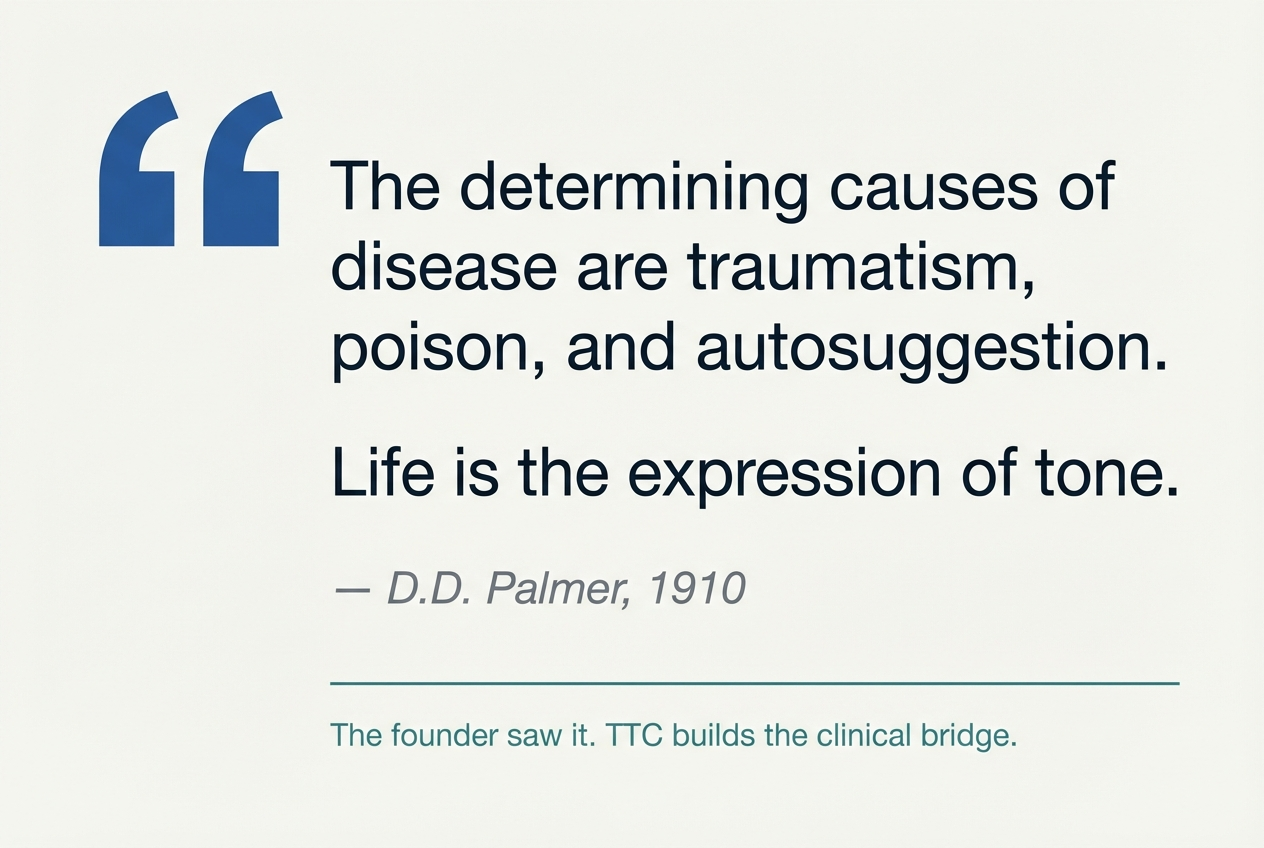
\includegraphics[width=0.65\textwidth]{18-dd-palmer-a-typographic.png}
\end{center}
\vfill
{\small\color{primaryblue!70}
\textit{``Life is an expression of tone; the cause of disease is any variation in tone.''}\\
\hspace*{2em}--- D.D.\ Palmer, \textit{The Chiropractor's Adjuster}, 1910\par}
\vspace{1cm}
\end{titlepage}

% Table of Contents
\clearpage
\setstretch{1.2}
\tableofcontents
\setstretch{1.4}
\clearpage







\section{Executive Summary}

\begin{figure}[htbp]
\centering
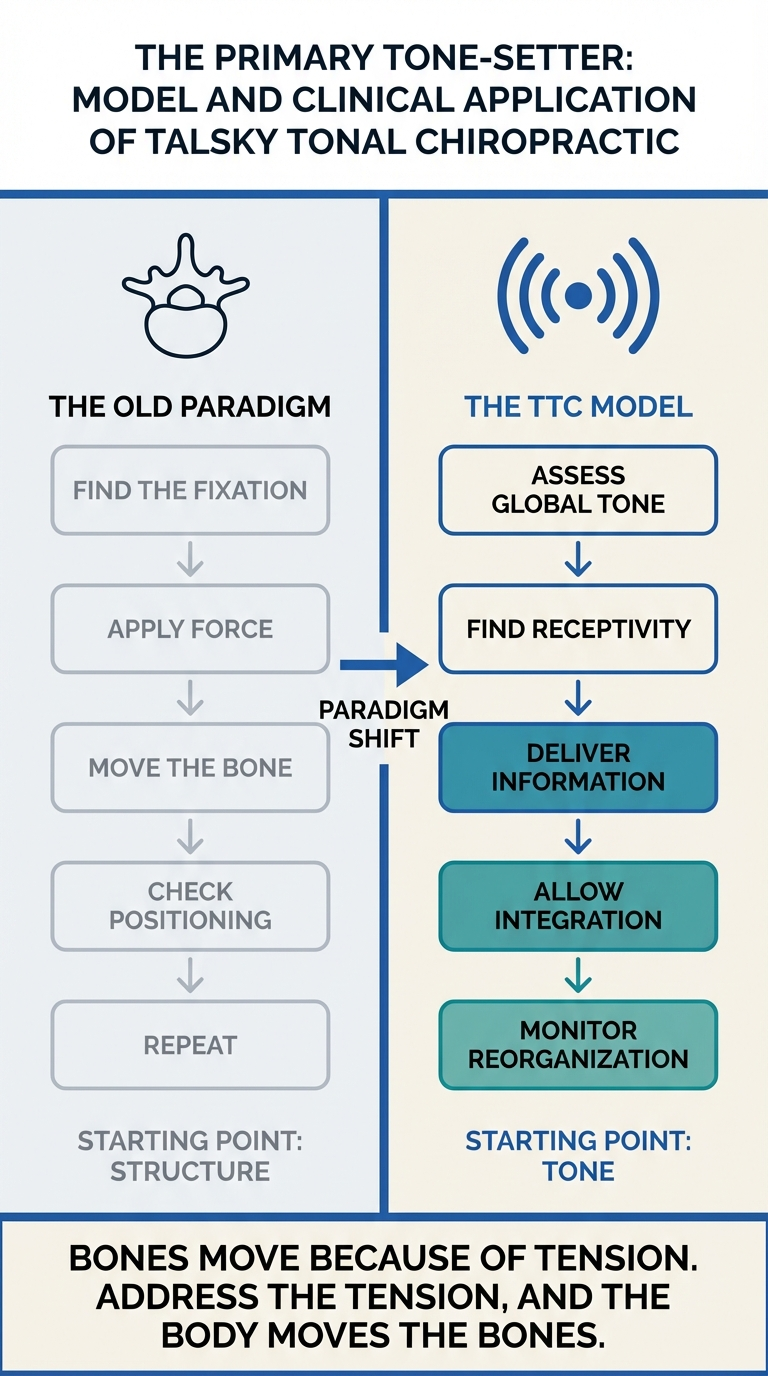
\includegraphics[width=0.85\textwidth]{08-summary-infographic-c-paradigm-shift.png}
\caption{TTC Paradigm Shift: Summary}
\end{figure}
\FloatBarrier



Every principled chiropractor has encountered the same clinical puzzle. A patient presents with clear vertebral subluxation. The adjustment is well-delivered. The segment moves. And yet the pattern returns within days, or never fully resolves. Meanwhile, another patient holds their correction for months. What is the difference?


Talsky Tonal Chiropractic (TTC) proposes a mechanism that accounts for this discrepancy: \textbf{vertebral subluxation is most accurately understood as a secondary, compensatory event.} The primary interference takes place upstream, in the NeuroSpinal System (Cranio-Spinal Meningeal Functional Unit), where sustained meningeal contracture alters the system's baseline tone. Muscles move bones; they hold them in compensatory positions as a result of core dural tension, not the other way around. TTC identifies the meningeal system as the \textbf{Primary Tone-Setter} — the structure whose baseline tension governs the global patterns that shape posture, adaptability, autonomic regulation, and the persistence of subluxation.


\textbf{Why this matters to your practice.} You have likely seen patients whose symptoms resolve without vertebral movement, and patients whose alignment looks clean on film but who cannot hold their health. TTC offers a framework for both phenomena. When the NeuroSpinal System is addressed directly, vertebral compensation often self-corrects because the upstream driver has been engaged. TTC does not replace the approaches you already use; it proposes the mechanism that determines whether any approach holds.


Prior tonal models made an important start: Epstein proposed the cord-meningeal system as the initiating site for Class B (facilitated) subluxation. TTC extends this further. In the TTC model, meningeal involvement is present across all subluxation classes — even Class A (physically traumatic) subluxation is sustained, in part, through meningeal contracture. The 5 D's cascade has a step upstream: aberrant NeuroSpinal tone. TTC is first a model and only second a technique, applicable across osseous, tonal, and combined approaches alike.


The mechanobiological framework presented here is anchored in established dural-muscular continuities (Scali et al., 2011) and myofibroblast contractility in meningeal tissue (Dorrier et al., 2021; Tomasek et al., 2002). Where the model proposes subclinical extensions of demonstrated pathological mechanisms, this is stated explicitly as TTC hypothesis throughout. The model is designed to be evaluated on anatomical plausibility, internal consistency, and testability.


\begin{pullquotebox}
"The NeuroSpinal System is the Primary Tone-Setter. Vertebral subluxation is the body's best available adaptation to that primary tonal disturbance."
\end{pullquotebox}


\section{First Principles}


Talsky Tonal Chiropractic (TTC) first and foremost returns to the original intent of chiropractic: the progressive reduction of physical interference to the physical nervous system maintained by incomplete and abnormal movement of spinal segments.


This foundational principle, championed by generations of principled chiropractors, recognizes that subluxation represents a state of interference that limits the body's capacity to express its full potential for health, adaptation, and self-regulation. The chiropractic profession has long held this truth at its center: that the integrity of the nervous system is paramount, and that interference must be addressed to restore the body's innate ability to heal and function optimally.


TTC honors this foundation while representing a profound shift in how we interact with the nervous system. Principled subluxation-based chiropractors are doctors of cause: we communicate with the body's intelligence to help it re-initiate its own process of subluxation reduction through chiropractic adjustments. TTC addresses the initiatory process, the upstream neurophysiology that gives rise to the Vertebral Subluxation Complex (VSC). TTC does not negate the VSC; it proposes a mechanism that initiates and maintains it.


\textbf{Standing on the shoulders of those who came before us.} No model emerges in isolation. The difference between stealing and evolution is clear: stealing takes what others have built, gives no credit, adds nothing new, and presents it as original. Inspiration and evolution, which is how all genuine advancement works, have two defining characteristics: giving credit to those who came before, and contributing something uniquely new. That new contribution is often not merely an improvement of what preceded it but a departure in a different direction — a new emphasis in analysis or application. The chiropractic profession needs this kind of divergence. There is a rich variety of chiropractors and an even richer variety of people in this world who so direly need our care. Divergence is a principle of evolution itself: picture the tree of chiropractic evolution as one whose branches divide and redivide as it grows. Whether a branch remains part of the tree is a matter of whether its divergence stays rooted in the principles of chiropractic.


Breig demonstrated that adverse mechanical tension in the meningeal system can disturb neural function without vertebral displacement. Ward brought Breig's insight into chiropractic practice, conceptualizing the spine as a unified meningeal-spinal unit. Epstein built on both, coining the Spinal Meningeal Functional Unit, distinguishing structural from facilitated subluxation, and synthesizing indicators from multiple techniques into the first integrated tonal clinical framework in chiropractic (see Part VI, Section 6.4 for the full account of these contributions). TTC stands on these shoulders and extends the work in directions that are distinct and new — detailed throughout Parts VI and VII.


\begin{pullquotebox}
"Divergence is a principle of evolution itself. Whether a branch remains part of the tree is a matter of whether its divergence stays rooted in the principles of chiropractic."
\end{pullquotebox}


\partbreak{Part I. From Principle to Clinical Method}{First Principles named the gap between chiropractic's philosophy and its practice. Part I closes that gap — describing what a clinical method looks like when it takes the intelligence of the nervous system literally.}

\begin{figure}[htbp]
\centering
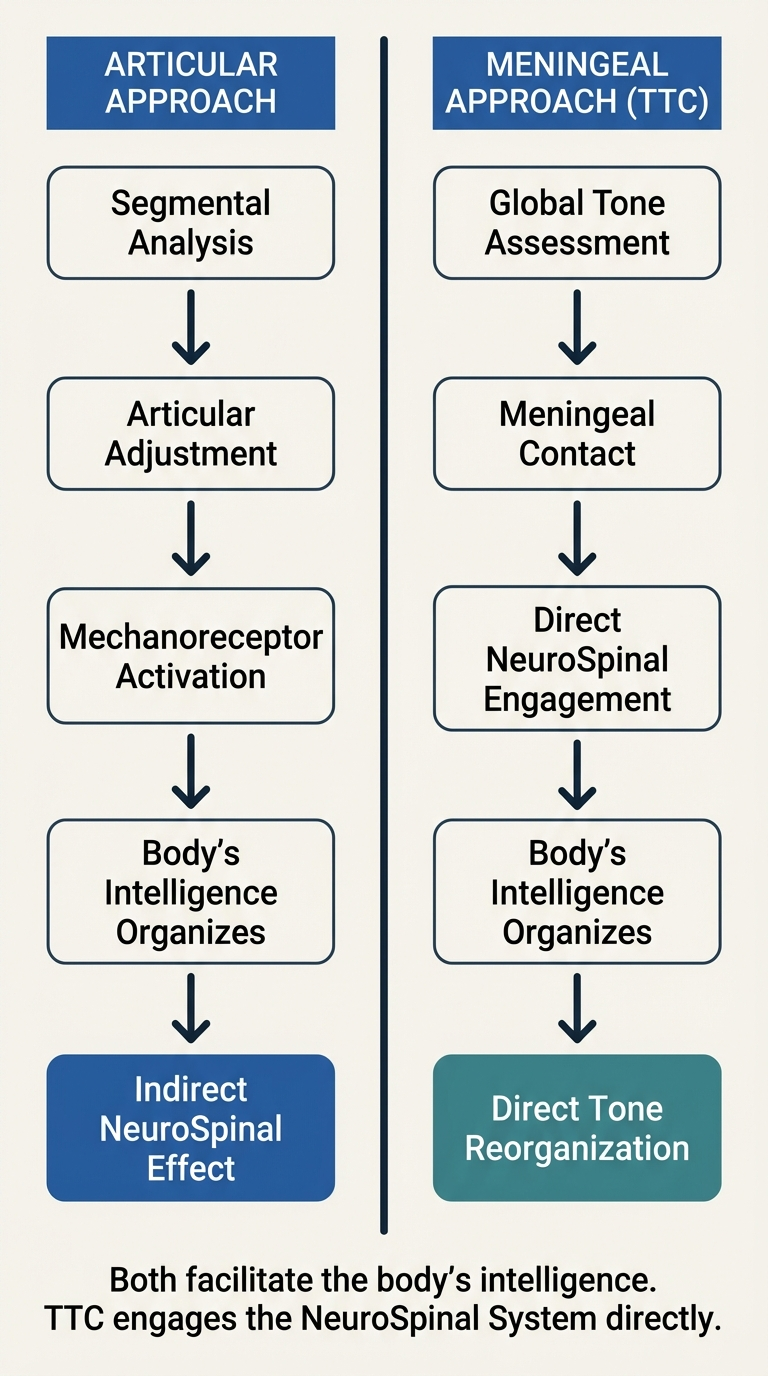
\includegraphics[width=0.85\textwidth]{01-concept-map-a-split-v2.png}
\caption{Bone-First vs.\ Tension-First: Two Paradigms of Subluxation}
\end{figure}
\FloatBarrier


\section{Part I. From Principle to Clinical Method}


Chiropractic was founded on the principle that life is an expression of tone and that interference to the nervous system limits that expression. Yet in daily practice the profession has overwhelmingly emphasized joint fixation, segmental malposition, and nerve compression while giving far less clinical attention to the nervous system's tone itself. \textbf{We said "tone," but we adjusted "bones." We said "intelligence," but we delivered force. We said "the body heals itself," but we delivered force to move bones rather than information to allow the body to move itself.} This is not a critique of structural methods, which can achieve meaningful clinical results. It is an observation about the gap between our explanatory language and our intervention model. This disconnect is the reason tonal approaches keep reappearing across decades. Chiropractors have always been trying to find the method that matches the philosophy.


\begin{pullquotebox}
"We said 'tone,' but we adjusted 'bones.' We said 'intelligence,' but we delivered force. We said 'the body heals itself,' but we delivered force to move bones rather than information to allow the body to move itself."
\end{pullquotebox}

The body is intelligent. The central nervous system is the chief coordinator, but it can only work with the information it receives. If interference is substantially mediated through altered tone, a tonal intervention may offer a more direct route of engagement than purely osseous methods. Talsky Tonal Chiropractic is an attempt to apply the original chiropractic principles to the actual structure that sets tone first.


When the NeuroSpinal System holds maladaptive tension beyond need, every subsystem must reorganize around that constraint: breath, gait, vestibular integration and gaze stabilization, sensorimotor coordination, autonomic regulation, and load management. This is not a local joint problem; it is global tensional dysregulation within the body's Primary Tone-Setter.


When incoming stress exceeds the body's adaptive capacity, the NeuroSpinal System tightens as an \textbf{allostatic response}, a protective adaptation that uses energy to maintain function under perceived stress. At first, this response is not pathological. It is an intelligent attempt by the body to stabilize itself and limit overwhelm. But as tone maintains and increases beyond actual need within the NeuroSpinal system, two key distortions emerge:


\begin{itemize}
\item \textbf{Misinformation} – Aberrant tension in the NeuroSpinal system alters afferent and efferent signaling.
\item \textbf{Missing information} – Increased NeuroSpinal tension restricts movement, narrowing the sensory input from proprioceptive and interoceptive pathways. This reduces the signal diversity and richness required for accurate regulation.
\end{itemize}

Together, these distortions impair the accuracy and clarity of communication between the brain and body. If the overload resolves, tone normalizes. But if it persists, \textbf{the system can no longer recognize safety}, and the protective pattern becomes maladaptive, laying the groundwork for vertebral compensation and eventual pathological changes in structure, function, and adaptability. (The full pathophysiology of this mechanism, including why it persists and how it is resolved, is described in Part IV.)


\begin{pullquotebox}
"If the overload resolves, tone normalizes. But if it persists, the system can no longer recognize safety, and the protective pattern becomes maladaptive."
\end{pullquotebox}

The spine is not just a column of separate joints. It is a tensioned, fluid-coupled, fascia-integrated, dura-anchored communication organ — mechanically continuous, richly innervated, and capable of influencing sensorimotor regulation throughout the body. In this framing, the NeuroSpinal System is not a passive unit of suspension; it is an active, self-tuning instrument animated by independent contractile motility of the meningeal system and the pulsatile dynamics of CSF.


TTC treats that proposition as literal. The work is not to force a vertebra to comply with a structural blueprint, but to offer precisely vectored information, delivered with focused intent, to the NeuroSpinal System so it can better perceive itself and resume its own corrective process. \textbf{We are not engaging the nervous system through joint mobilization or osseous thrusts.} Instead, TTC delivers precise, non-articular communication through touch to the soft tissue and meningeal system, communicating directly with the tone and tension of the NeuroSpinal System.


\textbf{Premise:} The intelligent system always seeks to self-correct; it is often missing accurate information, which tonal inputs are designed to provide.


\textbf{Intent:} Contact is made with the intent to communicate with the body's organizing intelligence through the physical matter of the nervous system.


\textbf{Location, Vector, and Timing:} Global tonal indicators guide the analysis; tonal pressure testing and leg balancing verify location, vector, and timing of input. We contact where the system confirms most receptivity, parallel to and opposite the direction of contraction — engaging the dura or its direct extension in the direction of release — and only when the system confirms receptivity. Between encounters, time is allowed for the body to process the adjustment.


\textbf{Amplitude and Quantity \textit{(Less is More)}:} The least amount of the most effective input, both in magnitude (enough to be heard, not enough to threaten or overpower) and number of contacts (enough to facilitate the body's response, not so many as to interfere with it).


We do not seek to apply force to what is stuck; \textbf{we seek to engage what is ready.} We are not looking for what's fixated; \textbf{we are looking for the best window in.} We are not looking for the most resistance; \textbf{we are looking for the most receptivity.}


\begin{pullquotebox}
"We do not seek to apply force to what is stuck. We seek to engage what is ready. We are not looking for the most resistance; we are looking for the most receptivity."
\end{pullquotebox}

Find the point of greatest receptivity and speak the language the system actually uses via tone, directional information, timing, and focused intent. We are not pushing bones into place; we are giving the body better information so it better perceives itself and its environment. The body communicates its response through whole-system balancing (leg checks or other balancing analyses). Outcome measures include improved adaptability, regulation, breathing ease, postural efficiency, and recovery after stress, indicators of the ongoing process of subluxation reduction.


\subsection{The Clinical Distinction}

\begin{figure}[htbp]
\centering
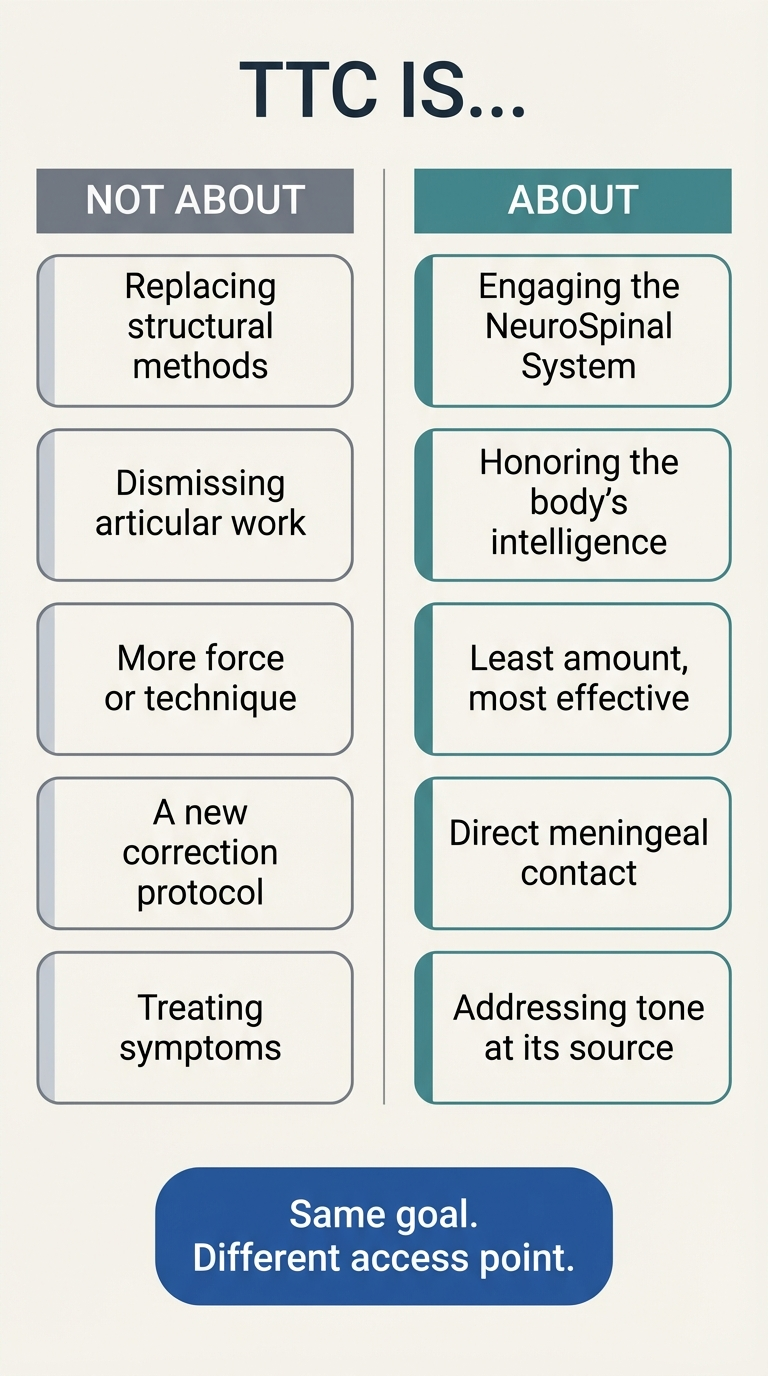
\includegraphics[width=0.85\textwidth]{11-not-about-a-two-column.png}
\caption{TTC IS\ldots\ A Paradigm Shift}
\end{figure}
\FloatBarrier


\begin{itemize}
\item \textbf{Not} about using enough force to move a bone, \textbf{about} delivering precise, minimal information to a system designed to self-correct.
\item \textbf{Not} about finding the primary fixation, \textbf{about} finding the best window in.
\item \textbf{Not} about joint cavitation, \textbf{about} re-toning a continuous meningeal instrument toward more optimally distributed tone.
\item \textbf{Not} about adding, moving, or manipulating energy, \textbf{about} precise analysis, focused intent, and physical inputs to the physical structures of the nervous system.
\item \textbf{About} identifying NeuroSpinal subluxation and practicing the philosophy, science, and art of facilitating the body to reduce subluxation through physical inputs with focused intent.
\item This distinguishes chiropractic's defining contribution to healthcare.
\item \textbf{Not} about maintenance as an endpoint, \textbf{about} ongoing improvement in neurological adaptability, regulation, and wholeness.
\end{itemize}

This is a move from localized segmental adjustments to the Tonal Model, engaging the NeuroSpinal System (C-SMFU) directly as the main functional unit through global tonal inputs that facilitate the body in its own adjustment process. It is not about us doing the adjusting; it is about engaging in a dialogue with the intelligence of the body through touch and intent, so that the system can resume its own process of releasing, resolving, and becoming more whole.


\subsection{Clinical Observations: Phenomena the Bone-First Model Struggles to Explain}

\begin{figure}[htbp]
\centering
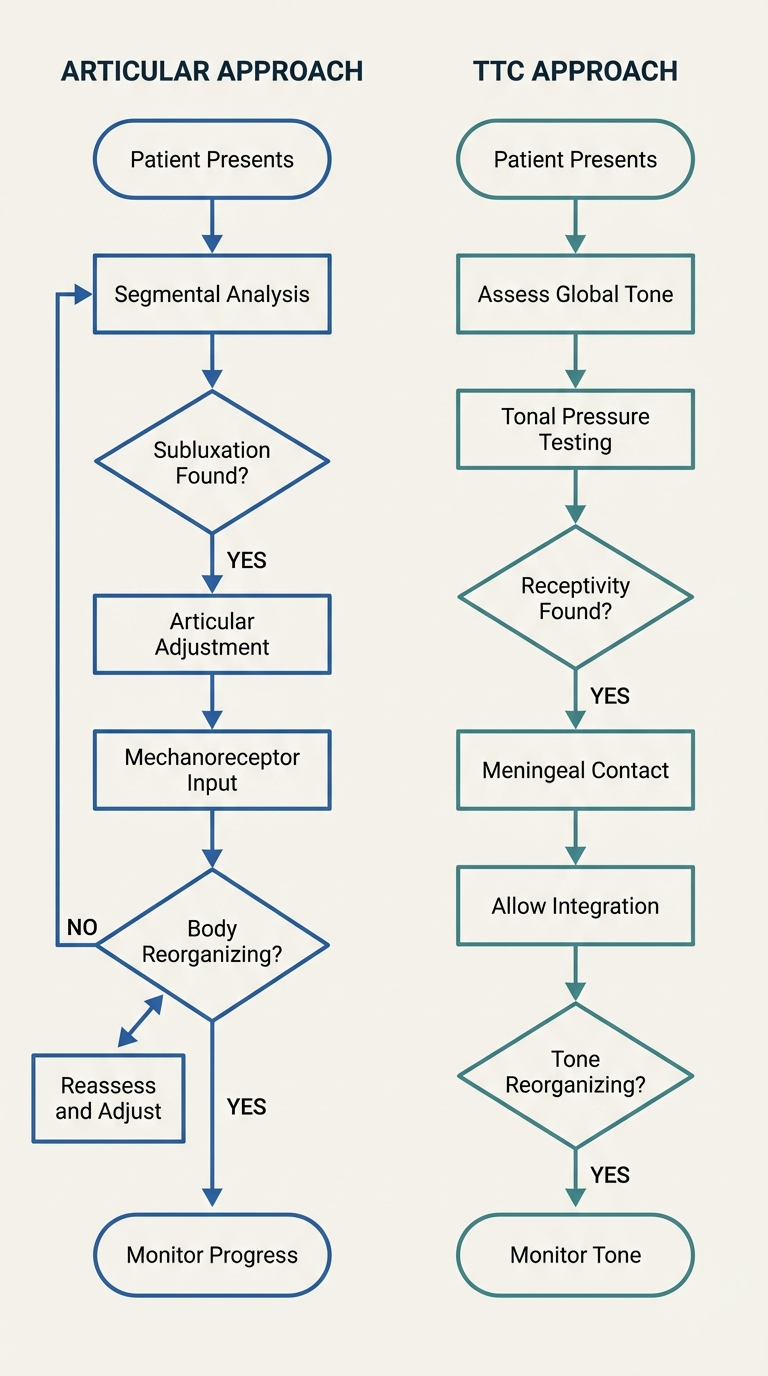
\includegraphics[width=0.85\textwidth]{03-clinical-flowchart-a-parallel-v2.png}
\caption{Traditional Chiropractic vs.\ TTC Clinical Pathway}
\end{figure}
\FloatBarrier


The following representative clinical scenarios illustrate patterns that principled chiropractors routinely observe but that the bone-first model does not fully account for. These are not individual case studies but composite observations drawn from clinical practice.


\begin{vignetteinner}
{\normalfont\bfseries Clinical Observation 1 — Improvement Without Measurable Vertebral Change}\\[4pt]
A patient presenting with chronic cervicogenic headaches and bilateral upper trapezius tension had been under care for several months. Repeat radiographic assessment showed no significant change in vertebral positioning from baseline. The practitioner, working through a tonal model, had been applying non-articular contacts at the occiput and C1 attachment sites with minimal force, guided by leg balance verification. Over the same period, the patient reported a 70\% reduction in headache frequency, improved sleep, and noticeably easier breathing. Nothing in the bony architecture had measurably changed. The primary structural outcome measure predicted no resolution.\\[2pt]
Traditional model prediction: Symptom resolution requires restoration of normal vertebral alignment; unchanged x-ray indicates insufficient correction.\\[2pt]
Observed outcome: Substantial symptom resolution with no measurable change in vertebral position.\\[2pt]
TTC interpretation: In the TTC model, vertebral position is a downstream compensation. When the primary NeuroSpinal tone is addressed directly, the nervous system can reorganize function without requiring visible structural change. The bones were never the driver; the aberrant tone was.\\[2pt]
\end{vignetteinner}


\begin{vignetteinner}
{\normalfont\bfseries Clinical Observation 2 — Normal Alignment, Persistent Dysfunction}\\[4pt]
A 38-year-old presenting with fatigue, postural collapse after moderate exertion, and recurring mid-thoracic pain had undergone full-spine radiographic workup showing alignment within normal parameters throughout the cervical, thoracic, and lumbar spine. No measurable vertebral misalignment was identified. Standard osseous analysis found minimal segmental fixation. The patient had received osseous adjustments at three clinics over two years with transient relief only. On tonal assessment, the practitioner identified persistent bilateral adduction resistance, a non-neutral breathing pattern anchored at the upper thorax rather than the sacrum, and notable thermal asymmetry at the craniocervical junction — all consistent with sustained aberrant NeuroSpinal tension despite unremarkable structural findings.\\[2pt]
Traditional model prediction: Normal alignment and minimal fixation should produce minimal dysfunction; the patient's presentation is unexplained by structural findings.\\[2pt]
Observed outcome: Persistent global dysfunction despite structurally normal radiographic and palpatory findings.\\[2pt]
TTC interpretation: In the TTC model, aberrant NeuroSpinal tone can exist and produce downstream dysfunction independently of vertebral position. The structural spine was not the problem; the NeuroSpinal System's maladaptive holding pattern was. Bones can be in place while tone remains profoundly disturbed.\\[2pt]
\end{vignetteinner}


\begin{vignetteinner}
{\normalfont\bfseries Clinical Observation 3 — Dramatic Response to Non-Osseous Contact After Repeated Osseous Failure}\\[4pt]
A patient with a long history of lumbar pain and intermittent lower extremity paresthesia had received high-velocity osseous adjustments consistently over 14 months at multiple practices, producing temporary relief of 24–72 hours' duration before symptoms returned. The pattern was stable: adjust, feel better, return to baseline. During a tonal assessment session, the practitioner identified that tonal pressure testing at the sacro-coccygeal junction, with a superior and slightly anterior vector, produced temporary bilateral leg length equalization. A non-articular contact at that site — minimal force, no articular movement — was held in the confirmed vector of release. Within the session, the patient's breathing pattern shifted from upper-thoracic to a full sacrum-to-occiput wave. At follow-up 72 hours later, the patient reported the longest pain-free interval of the preceding year.\\[2pt]
Traditional model prediction: Non-articular contact produces no structural change and should not be expected to outlast prior osseous interventions.\\[2pt]
Observed outcome: A non-osseous contact at the sacro-coccygeal dural attachment, precisely vectored through tonal pressure testing, produced a durable response that 14 months of osseous adjusting had not.\\[2pt]
TTC interpretation: In the TTC model, the repeated osseous adjustments had been engaging the body's compensatory layers without reaching the primary NeuroSpinal holding pattern. When the practitioner found the best window in, delivered precise directional information parallel to the aberrant dural tension, and the NeuroSpinal System received the safety signal it was waiting for, the protective meningeal contracture began to release — and the compensatory lumbar pattern with it.\\[2pt]
\end{vignetteinner}


\partbreak{Part II. The NeuroSpinal System}{Part I established why the tonal approach exists. Part II establishes what it is working with — the anatomy, contractility, and information-processing capacity of the system TTC treats as the body's primary tone-setter.}

\begin{figure}[htbp]
\centering
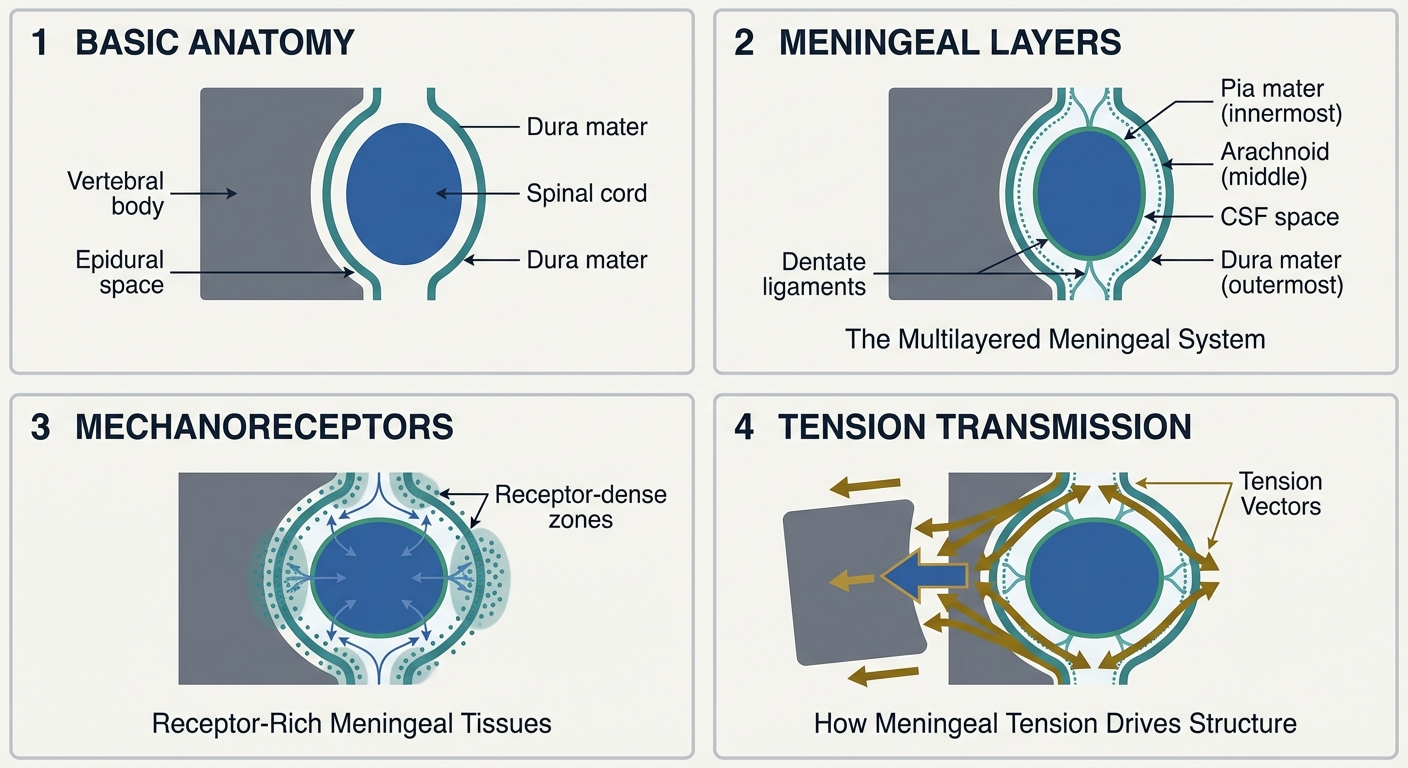
\includegraphics[width=0.85\textwidth]{05-meningeal-anatomy-a-four-panel-v2.png}
\caption{Meningeal Anatomy: The NeuroSpinal System}
\end{figure}
\FloatBarrier


\section{Part II. The NeuroSpinal System (Cranio-Spinal Meningeal Functional Unit)}



\subsection{Terminology Note}

Donald Epstein, D.C. introduced the term \textbf{Spinal Meningeal Functional Unit (SMFU)} to describe the cord-meningeal system as a unified clinical entity (Epstein, 1986). TTC extends this concept to the \textbf{Cranio-Spinal Meningeal Functional Unit (C-SMFU)}, emphasizing the cranial pole of the system (sphenoid, zygoma, occiput) alongside the spinal and sacral attachments, and reframing it as the body's Primary Tone-Setter. Throughout this paper, \textit{NeuroSpinal System} and \textit{Cranio-Spinal Meningeal Functional Unit (C-SMFU)} are used interchangeably. We retain both terms to reflect their functional unity and ensure clarity for professionals within and beyond the chiropractic field.


\subsection{Structural Composition}

The NeuroSpinal System comprises:


\begin{enumerate}
\item \textbf{Brain and spinal cord}
\end{enumerate}

\begin{enumerate}
\item \textbf{Pia mater:} Innermost meningeal layer, including the dentate ligament
\end{enumerate}

\begin{enumerate}
\item \textbf{Arachnoid space:} Including the cerebrospinal fluid that fills the space, a dynamic medium for signaling and pressure exchange
\end{enumerate}

\begin{enumerate}
\item \textbf{Dura mater:} Outermost meningeal layer, with clinical emphasis on the attachments to the movable bony structures of the cranium and spine.
\end{enumerate}

\textbf{Clinically significant areas of either direct or indirect dural attachments include:} Sphenoid, Zygoma, Occiput, C1, C2, C5, S1-S5, and Coccyx (see Appendix A for additional clinically relevant areas)


\begin{enumerate}
\item \textbf{Continuity:} The dural system extends its tensional field beyond the spinal canal through the outer dural sheath, periosteum, and connective tissue bridges, including myodural bridges connecting suboccipital musculature directly to the spinal dura (Scali et al., 2011; Zheng et al., 2014)
\end{enumerate}

\begin{evidencebox}
{\normalfont\bfseries Evidence Snapshot: Myodural Bridge}\\[3pt]
The myodural bridge connects suboccipital musculature directly to the spinal dura mater. Research suggests this connection may serve as an active and passive tension-monitoring system between movement and the central nervous system (Liu et al., 2017). These anatomical connections suggest the NeuroSpinal System extends its influence beyond the spinal canal through direct dural-muscular continuities.\par
\end{evidencebox}

This functions as a single organ of tension and transmission: the NeuroSpinal System mechanically unites the brain, spinal cord, and multilayered meningeal system with their attachments to the movable bony structures of the cranium and spine. The outer dural sheath extends continuously into the surrounding fascial network, positioning the NeuroSpinal System as a primary tone-setter for the body's fascia as well. In the TTC model, this system behaves as a \textbf{tensegrity lattice}, dynamically modulating CSF dynamics and global posture.


\subsection{Intrinsic Contractile Motility and Tone Generation}

\textbf{This system is not passive; it is active, dynamic, and independently motile.}


The multi-layered meningeal system acts as an active communication transfer mechanism to and from the CNS, predominantly through non-synaptic pathways. This system possesses independent contractile motility and is in constant motion, modulating its tone moment to moment as it continuously assesses and responds to changes in tension, movement, and the perception of threat.


\begin{pullquotebox}
"This system is not passive; it is active, dynamic, and independently motile. It autonomously sets its own tone, compelling muscles, fascia, joints, and posture to compensate around it."
\end{pullquotebox}

As Breig (1978) demonstrated, aberrant tension in the meningeal system can disturb neural function without vertebral displacement (see Part VI, Section 6.2 for the full historical account). Research has demonstrated fibroblast-to-myofibroblast differentiation in meningeal tissue, with \textbf{α-SMA–positive myofibroblasts} identified in the arachnoid membrane under pathological conditions (Dorrier et al., 2021; Fede et al., 2018). While direct investigation of meningeal myofibroblast activity under routine physiological stress is limited, these findings confirm that the meningeal system possesses intrinsic contractile capacity. The TTC model proposes that this mechanism also operates under chronic subclinical stress, providing the contractile force that generates and sustains aberrant NeuroSpinal tension.


Though the NeuroSpinal System is not a skeletal muscle, it \textbf{autonomously sets its own tone}, compelling muscles, fascia, joints, and posture to compensate around it. It actively contracts under actual or perceived stress, and expands and relaxes as the perception of stress resolves.


\textbf{Because of this dynamic responsiveness, TTC identifies the meningeal system as the Primary Tone-Setter in the body}, the structure whose baseline tension governs the global patterns that shape adaptability, breath, posture, energy, and regulation.


\subsection{Information Transmission, Reception, and Storage}

The NeuroSpinal System is not simply a structural framework; it is an \textbf{information processing continuum}:


\textbf{A. Transmission}: The dura and fascial network conduct mechanical and bioelectrical signals throughout the body. As synthesized by Becker and Selden (1985), connective tissue may function as a communication system operating alongside traditional neural pathways. One established mechanism underlying this capacity is \textbf{piezoelectric signal transduction}: collagen, the primary structural protein in fascia and dura, generates electrical charge in response to mechanical stress (Fukada \& Yasuda, 1964), enabling mechano-electric conversion between tissue layers and neural structures. While the biological significance of collagen piezoelectricity remains an area of active investigation, this property provides a plausible pathway for non-synaptic mechanical signaling within the meningeo-fascial continuum.


\textbf{B. Reception}: Mechanoreceptors embedded in the meningeal layers respond to tension, movement, and pressure, feeding real-time proprioceptive data into the central nervous system.


\textbf{C. Storage}: Emerging research suggests that fascia undergoes persistent mechanical and phenotypic changes after loading history: patterns of altered stiffness and extracellular matrix remodeling that persist after the original stressor has resolved, influencing future tissue behavior (Fede et al., 2018). The TTC model extends this concept to meningeal tissues, which share structural characteristics with fascia and have demonstrated sustained phenotypic changes under chronic mechanical stress.


\textbf{Working hypothesis}: The NeuroSpinal System functions as a high-bandwidth, analogue-digital interface that regulates the tone through which Innate Intelligence coordinates global adaptation.


\subsection{The NeuroSpinal System as the Fountainhead of Tone}

If tone is the organizing principle of life, as D.D. Palmer proposed, then this paper proposes that the NeuroSpinal System is the \textbf{Primary Tone-Setter} of the human body.


When stress overloads the system, the meningeal system contracts protectively (see Part IV for the full mechanism). This increases baseline tension in the NeuroSpinal continuum. The brain perceives this aberrant tension and responds by commanding compensatory muscle patterns, which pull on bony structures, creating postural shifts, gait disturbances, and joint fixations — initiating the cascade of dyskinesia, dysafferentation, dysponesis, dysautonomia, and degeneration (each defined in Part IV).


Muscles move bones and hold them in their positions as a result of core dural tension, not the other way around. While osseous approaches can achieve meaningful changes when they influence the underlying NeuroSpinal tone — working through mechanoreceptor-rich joint spaces to engage the body's intelligence — TTC engages the NeuroSpinal System directly through the most receptive dural contacts.


\begin{pullquotebox}
"Muscles move bones and hold them in their positions as a result of core dural tension, not the other way around."
\end{pullquotebox}

The anatomy described above is not speculative. A growing body of peer-reviewed research supports the meningeal system's contractile capacity, the myodural bridge's clinical significance, and the neurophysiological effects of tonal chiropractic inputs. The following evidence map surveys this foundation and identifies the research questions TTC is positioned to answer.


\section{Part III. Evidence Map and Research Invitations}



\subsection{On Intent and Information}

Living systems are exquisitely sensitive to boundary conditions and small inputs. Contextual factors, including practitioner attentional quality, touch modulation, confidence, therapeutic alliance, and focused intent, demonstrably influence clinical outcomes through well-established neurophysiologic pathways involving expectancy effects and contextual modulation.


When the body is listening, the coherence between your focused intent and your physical input can amplify the effectiveness of the adjustment. Focused intent, what B.J. Palmer called "that something extra," enhances signal fidelity in a living system designed to detect and respond to information. While the physical input remains the primary mechanism, the alignment of intent with action strengthens the neurological communication that facilitates the body's corrective process. (For practitioners interested in exploring the broader body of research on intent and information, including exploratory work on mind-matter interaction, see Appendix B.)


\begin{pullquotebox}
"Living systems are exquisitely sensitive to boundary conditions and small inputs. When the body is listening, the coherence between your focused intent and your physical input can amplify the effectiveness of the adjustment."
\end{pullquotebox}


\subsection{Research Priorities}

TTC's clinical effects are compelling, but its mechanisms demand deeper investigation. The non-articular nature of TTC offers unique research opportunities to isolate the meningeal-dural pathway's contribution to the neurophysiological changes documented in chiropractic research.


Dr. Heidi Haavik's research has shown that chiropractic adjustments of dysfunctional spinal segments produce measurable changes in brain function. A brain source localization study estimated changes of nearly 20\% in prefrontal cortex processing (Lelic et al., 2016), with the caveat that brain source localization is an indirect measurement method and the study's findings await replication with larger samples. Importantly, Haavik's research protocols employed articular spinal manipulation (HVLA), not non-articular tonal contacts. Her established protocols using somatosensory evoked potentials (SEPs), fMRI, and transcranial magnetic stimulation (TMS) could be applied to TTC to investigate whether non-articular tonal contacts produce comparable or distinct neurological changes compared to articular approaches.


\subsection{The Need for Clinical Outcomes Research}

To date, no published controlled trials have isolated TTC methodology from other approaches. While the mechanistic foundation draws on multiple lines of peer-reviewed research and clinical observations are compelling, rigorous outcomes research is needed to quantify TTC's effects on autonomic regulation, postural adaptation, and long-term neuroplasticity. This represents the next critical step in validating the model.


\begin{pullquotebox}
"To date, no published controlled trials have isolated TTC methodology from other approaches. While the mechanistic foundation draws on multiple lines of peer-reviewed research and clinical observations are compelling, rigorous outcomes research is needed."
\end{pullquotebox}


\subsection{Limitations and Future Directions}

\textbf{Model Limitations:}

This model synthesizes existing research from multiple fields but has not yet been tested as an integrated framework. The proposed mechanisms draw on fascial research, meningeal tissue biology, neuroscience, and chiropractic studies, but direct investigation of TTC-specific pathways is needed. Recent meta-analytic evidence (2025) suggests that spinal manipulation outcomes may not depend strongly on application procedures, region of application, or site specificity, a finding that, while based primarily on HVLA thrust techniques, challenges the premise that TTC's precise location, vector, and timing produce superior outcomes through a distinct mechanism. Demonstrating that TTC's site-specific methodology produces measurably different results from non-specific approaches remains a critical research priority.


Additionally, while this model proposes that meningeal involvement is present in all subluxation, including cases where direct mechanical compression is well-documented (e.g., disc herniation, foraminal stenosis), TTC does not deny the reality of pathological compression. Rather, TTC proposes that even where compression exists, there is associated tension within the meningeal system that preceded or accompanies the structural event, and that addressing this meningeal component directly facilitates the body's own process of resolving the dyskinesia.


\textbf{Research Priorities:}

\begin{enumerate}
\item Controlled trials comparing TTC to other tonal and osseous approaches, including non-specific manipulation controls
\item Neuroimaging studies using Haavik's protocols to measure whether non-articular tonal contacts produce distinct cortical effects from articular manipulation
\item Mechanistic studies isolating the meningeal-dural pathway contribution
\item Investigation of meningeal myofibroblast activity under chronic subclinical stress (extending current pathological findings to the physiological context TTC proposes)
\item Long-term neuroplasticity outcomes with sustained TTC care
\item Investigation of focused intent as a measurable variable in clinical outcomes
\end{enumerate}

The anatomical and neurophysiological evidence establishes that the meningeal system is active, contractile, and clinically significant. The mechanism by which it initiates subluxation — and why that pattern persists — is the subject of Part IV. To the authors' knowledge, this is the first mechanobiological account within chiropractic of why meningeal contraction begins, how it is sustained at the cellular level, and what conditions allow it to release.


\section{Part IV. Pathophysiology of NeuroSpinal Subluxation}

\begin{figure}[htbp]
\centering
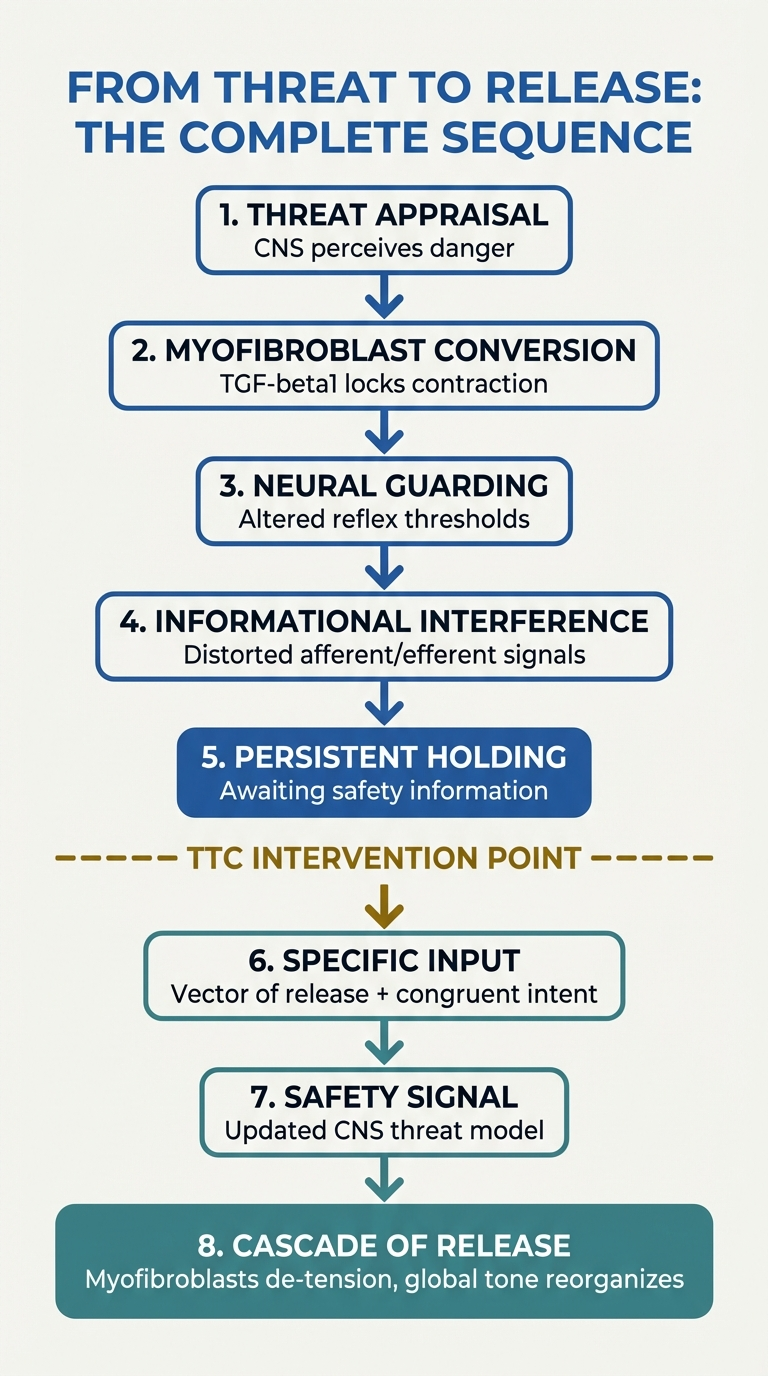
\includegraphics[width=0.85\textwidth]{09-five-ds-cascade-c-threat-to-release.png}
\caption{The 5 D's Cascade: From Threat Perception to Release}
\end{figure}
\FloatBarrier



Previous tonal models identified the clinical phenomenon; this section presents the underlying biology. To the authors' knowledge, this is the first mechanobiological model within chiropractic explaining why the meningeal system contracts, how that contraction persists at the cellular level, and what allows release to occur. In doing so, this section describes the neurophysiology of the initiation of subluxation, the process of its reduction, and most importantly, the chiropractor's role in facilitating the body to re-initiate its own process of subluxation reduction.


\subsection{The Protective Meningeal Response and Development of Aberrant NeuroSpinal Tension}

Subluxation begins upstream of joint fixation. The initiating event is often the perception of threat, whether actual or imagined. This appraisal, processed by cortical and limbic structures, triggers a protective meningeal contraction in the NeuroSpinal System.


This protective response involves active contractility of the meninges, particularly via the pia mater and dentate ligaments, reinforced by dural-muscular connections such as the myodural bridge (Scali et al., 2011). When the NeuroSpinal System, the body's Primary Tone-Setter, locks into persistent meningeal contracture, creating aberrant NeuroSpinal tension, it operates through three interrelated mechanisms:


\textbf{Mechanobiology:} Under sustained load, mechanotransduction shifts fibroblasts toward myofibroblast behavior through TGF-β1 signaling, embedding α-SMA fibers that sustain contraction and alter extracellular matrix tone (Tomasek et al., 2002; Wipff et al., 2007). In pathological contexts, fibroblast-to-myofibroblast differentiation with α-SMA expression has been demonstrated in the arachnoid membrane, driven by elevated TGF-β1 concentrations in cerebrospinal fluid (Dorrier et al., 2021). These findings confirm that meningeal tissue possesses intrinsic fibrotic and contractile potential. TTC hypothesizes that lower-grade analogues of this mechanism may operate under chronic subclinical stress, but this specific extension from pathological to routine physiological contexts has not been directly demonstrated.


\textbf{Altered Afference:} Sensory input from dural and periosteal tissues changes the baseline signals arriving in the brainstem and higher centers, biasing central processing and motor planning. Mechanoreceptors in tense meningeal tissues send repetitive, low-resolution data to the CNS, limiting adaptability.


\textbf{CSF Hydrodynamics:} The pulse, swirl, and return dynamics of cerebrospinal fluid may be influenced, affecting pressure exchange and chemical signaling throughout the neuraxis (Brinker et al., 2014; Alperin et al., 2000). Strain alters axoplasmic flow and CSF dynamics, reducing nutrient/waste exchange.


The result is a systemic change in the default tensional set-point of the NeuroSpinal System. Many downstream structural findings (postural compensations, joint restrictions, muscle hypertonicity, and vertebral subluxation) become effects, not primaries. Addressing the primary tone allows for more lasting change.


\subsubsection{The Cascade of Dysfunction}

When aberrant NeuroSpinal tone persists, it initiates a progressive cascade of downstream consequences:


\begin{itemize}
\item \textbf{Dyskinesia}: Movement dysfunction arising from altered motor output and compensatory postural strategies
\item \textbf{Dysafferentation}: Distorted sensory input from aberrant mechanoreceptor activity in tense meningeal tissues, reducing the fidelity of proprioceptive and interoceptive data
\item \textbf{Dysponesis}: Misdirected neurological effort: inappropriate muscle activation patterns that waste energy and reinforce compensatory holding
\item \textbf{Dysautonomia}: Autonomic dysregulation resulting from sustained sympathetic bias and narrowed adaptive bandwidth
\item \textbf{Degeneration}: Progressive structural and functional decline from chronic maladaptation, as tissues remodel around the persistent aberrant tone
\end{itemize}

This cascade is not linear but self-reinforcing: each stage deepens the conditions that sustain the others, making spontaneous resolution increasingly unlikely without specific input to the Primary Tone-Setter.


\begin{pullquotebox}
"This cascade is not linear but self-reinforcing: each stage deepens the conditions that sustain the others, making spontaneous resolution increasingly unlikely without specific input to the Primary Tone-Setter."
\end{pullquotebox}


\subsubsection{Informational Interference Under Sustained Tone}

While protective tone is held, informational flow through the NeuroSpinal System is altered at multiple levels:


\begin{itemize}
\item \textbf{Afferent Distortion}: Mechanoreceptors in tense meningeal tissues send repetitive, low-resolution data to the CNS, limiting the system's ability to perceive its environment accurately and respond adaptively.
\item \textbf{Conduction and Transport Impedance}: Sustained strain alters axoplasmic flow and CSF dynamics, reducing nutrient and waste exchange and degrading the efficiency of signal transmission along neural pathways.
\item \textbf{Central Processing Bias}: Chronic sympathetic activation narrows cortical resources toward threat detection, while neuroinflammation may further reduce neuroplasticity and adaptive capacity.
\item \textbf{Descending Control Default}: Poor-quality afferent input biases efferent output toward sustained guarding, reinforcing the protective holding pattern from above.
\end{itemize}

Together, these mechanisms create both misinformation (skewed data from aberrant mechanoreceptor activity) and missing information (silenced pathways due to restricted movement), further reinforcing the need for the defensive holding pattern.


\subsection{Why Aberrant NeuroSpinal Tension Persists: The Persistence of Meningeal Contracture}

\textbf{This is the mechanism the TTC model proposes as fundamental to both the initiation of subluxation and the process of subluxation reduction:}


\textbf{Critically, meningeal contracture and the resulting aberrant NeuroSpinal tension persist long after the original stressor is gone.} The meningeal system does not automatically release when the threat dissipates. Instead, it maintains this defensive holding pattern, this aberrant tension, until specific conditions are met: (1) mechanical input through directional movement that addresses the restricted tissue, (2) activation of mechanoreceptors within the fascial-meningeal continuum, and (3) parasympathetic nervous system activation signaling safety (Schleip, 2003; Schleip \& Müller, 2013; Bordoni \& Zanier, 2013; Wipff et al., 2007; McHugh et al., 1998).


The mechanism parallels the flexibility phenomenon seen under anesthesia (McHugh et al., 1998):


\begin{itemize}
\item \textbf{Awake:} The CNS limits range-of-motion (e.g., hamstring stretch) to protect against predicted harm through protective muscle contraction and neural mechanosensitivity.
\end{itemize}

\begin{itemize}
\item \textbf{Under anesthesia:} Protective tone vanishes, research shows significant increases in range of motion without tissue damage, revealing that the limitation was neural, not structural.
\end{itemize}

The limitation is neural, not structural. The tissue itself is capable of greater range, but the nervous system restricts it as a protective strategy. Similarly, in subluxation, protective meningeal tone persists, held as stored potential, until the system experiences directional movement in the vector of release without concurrent stress signaling. This provides the safety signal the nervous system needs to release the held contraction and allow the system to begin self-correcting.


\subsubsection{Why the Contracture Persists After Stress Resolves}

\textbf{1. Myofibroblast Phenotype Stability}


Once fibroblasts differentiate into myofibroblasts through TGF-β1 signaling and mechanical load, they maintain their contractile phenotype until receiving specific biochemical and mechanical signals to reverse (Wipff et al., 2007). The α-SMA fibers embedded in these cells create sustained contractile capacity that does not simply "turn off" when the external threat is removed.


\textbf{2. Lack of Safety Information}

The nervous system continues to operate under the original threat model (Woo et al., 2017). Without clear informational input signaling safety (specifically, the experience of safe movement through the restricted range), the protective pattern remains active. The CNS has not received the data it needs to update its internal model and conclude that the defensive posture is no longer necessary.


\textbf{3. Movement Restriction Creates Self-Reinforcing Cycle}

The contracture itself limits the range of motion needed to generate the sensory feedback that would signal safety (Schleip, 2003; McHugh et al., 1998). This creates a self-perpetuating loop: the system restricts movement to protect itself, but that very restriction prevents it from gathering the sensory information (safe movement through previously restricted ranges) that would allow it to release the protection.


\textbf{4. Stored Adaptive Pattern}

Research suggests that the body may retain the protective strategy as a stored adaptive pattern (Fede et al., 2018). This held tension represents stored potential, an adaptive pattern that served a purpose during the acute threat but has become maladaptive in its persistence. The pattern is held in the tissue as both mechanical tension and as an informational state within the nervous system.


\textbf{The body is waiting for the safety signal to release, which comes through experiencing safe, directional movement parallel to the line of release.}


\begin{pullquotebox}
"The body is waiting for the safety signal to release, which comes through experiencing safe, directional movement parallel to the line of release."
\end{pullquotebox}


\subsubsection{Why Precision Matters: Layers of Tension and the Best Window In}

\begin{figure}[htbp]
\centering
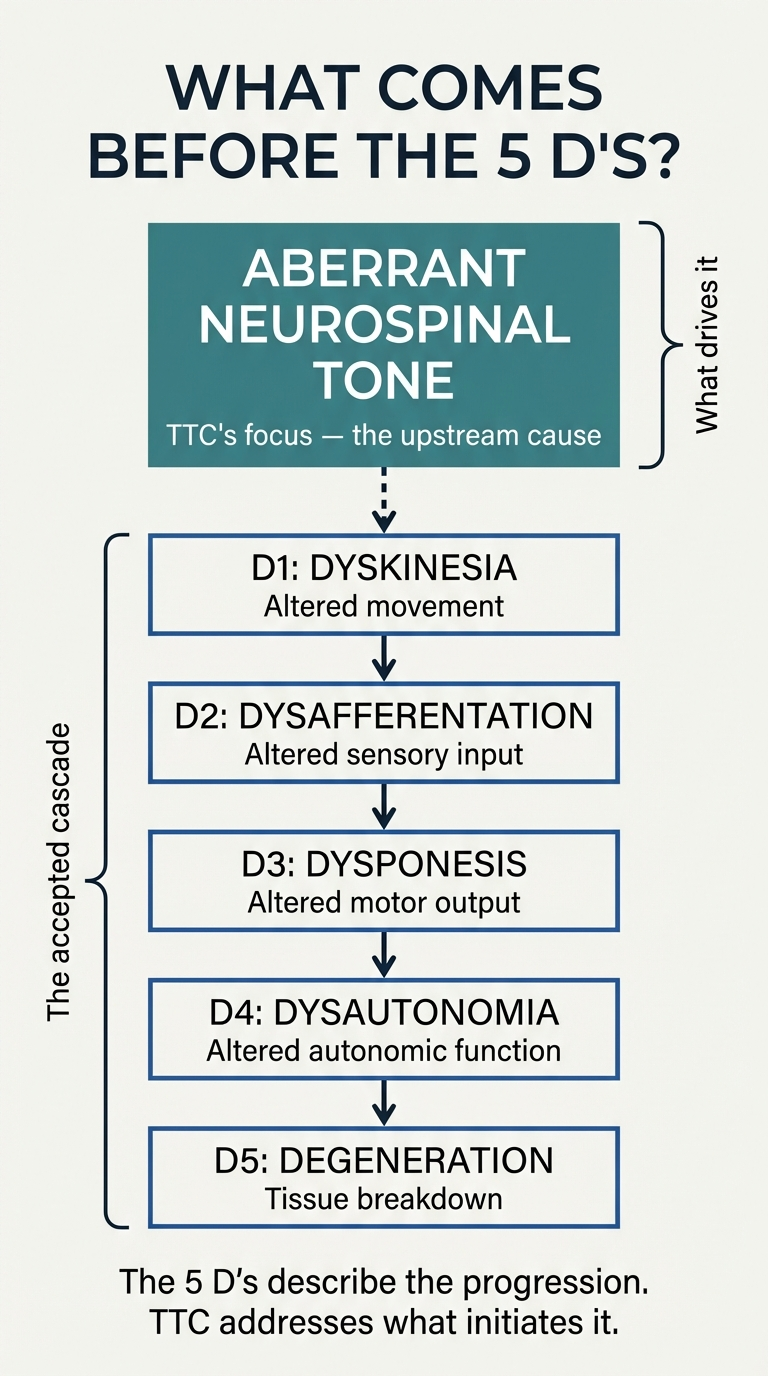
\includegraphics[width=0.85\textwidth]{19-upstream-a-cascade.png}
\caption{Upstream Insight: Aberrant NeuroSpinal Tension Precedes the 5 D's}
\end{figure}
\FloatBarrier


If simple movement or stretching were sufficient to release these patterns, far more subluxations would self-resolve through daily activity. Many do not. The reason lies in the \textbf{layered architecture of compensatory tension} that accumulates around the primary NeuroSpinal restriction.


When the NeuroSpinal System contracts defensively, the body does not experience this tension as a singular, isolated phenomenon. Instead, it organizes \textbf{multiple compensatory layers} around the primary restriction:


\begin{itemize}
\item \textbf{Global postural shifts} to redistribute load away from the area of greatest tension
\item \textbf{Regional soft tissue bracing} creating secondary restrictions
\item \textbf{Local joint fixations} as vertebrae lock into positions that minimize stress on the contracted meningeal system
\item \textbf{Protective muscle guarding} layered over all of the above
\end{itemize}

Each layer represents the body's intelligent attempt to protect the core restriction. But these compensatory layers also \textbf{obscure the primary pattern} and create a maze of tension that gross movement cannot penetrate. General range of motion exercises engage the outer compensatory layers without addressing the core NeuroSpinal holding pattern. The system remains in its protective stance because the Primary Tone-Setter (the NeuroSpinal System itself) has not received the specific directional information it needs to release.


\textbf{This is why finding the best window in is essential.} Through tonal pressure testing verified by leg balancing, the practitioner identifies the precise location and vector where the NeuroSpinal System demonstrates receptivity, where the layers of compensation momentarily align to create a clear pathway to the core pattern. When balanced legs are observed, TTC interprets this as a clinical indicator that \textbf{this specific contact, in this specific direction, at this specific time} offers a pathway to the primary holding pattern.


\textbf{This is why the least amount of the most effective input works when gross force does not.} TTC hypothesizes that precise, low-force input (parallel to the line of release, delivered with focused intent, at the confirmed point of receptivity) may preferentially engage the most clinically relevant layer of the compensatory pattern. This specific directional information, received without triggering a stress response, provides the safety signal the system has been waiting for. It allows the Primary Tone-Setter to release its defensive holding pattern, which then allows the compensatory layers to release in cascade.


The body does not need more mechanical input; it needs \textbf{the right mechanical input, delivered at the right place, in the right direction, at the right time, with congruent intent}. This is what allows the nervous system to begin releasing held tension and reducing subluxation on its own. TTC's methodology speaks the precise language the NeuroSpinal System uses to govern tone and coordinate self-adjustment.


\begin{pullquotebox}
"The body does not need more mechanical input; it needs the right mechanical input, delivered at the right place, in the right direction, at the right time, with congruent intent."
\end{pullquotebox}


\subsubsection{Why Force Isn't the Language of Change}

In a system regulated by information bandwidth, more force does not equal more effectiveness; it equals more noise. When the NeuroSpinal System is already in a defensive pattern, high-threshold input can reinforce the bracing response, bypass the actual tone generator (the NeuroSpinal System itself), and trigger protective compensation rather than authentic reorganization. The body's intelligence expresses through tone, and tone listens through touch. The adjustment is not about force; it is about signal integrity: delivering a coherent input through the right window so that the system receives the information it needs to release and reorganize.


\subsection{The Sequence: From Threat to Release}

\begin{enumerate}
\item \textbf{Threat Appraisal:} CNS perceives danger → meningeal contraction
\item \textbf{Fibroblast → Myofibroblast Conversion:} Sustained load and TGF-β1 lock in contractile phenotype
\item \textbf{Neural Guarding:} Increased gamma motor gain, altered reflex thresholds
\item \textbf{Informational Interference:} Reduced variability and fidelity of afferent/efferent signals (misinformation + missing information)
\item \textbf{Persistent Holding Pattern:} Contracture maintained long after stressor resolves, awaiting safety information
\item \textbf{Specific Input in Vector of Unwinding:} Precise mechanical + intentional congruence delivered parallel to tension
\item \textbf{Safety Signal Integration:} Updated CNS threat model → parasympathetic shift
\item \textbf{Cascade of Release:} Myofibroblasts de-tension → dural slack returns → global tone reorganizes
\end{enumerate}

\textbf{Key Principle:}

\textit{TTC is not about forcing tissue change but delivering precisely enough information for the system to choose reorganization and resume its own corrective process.}


\begin{pullquotebox}
"TTC is not about forcing tissue change but delivering precisely enough information for the system to choose reorganization and resume its own corrective process."
\end{pullquotebox}


\subsection{Visual Model: Aberrant NeuroSpinal Tension and Release Pathways}

\textbf{Protective Meningeal Contraction is the Primary Mechanism:}


\begin{verbatim}
CLASS B (Facilitated Subluxation):
Threat Perception
  ↓
Protective Meningeal Contraction → Aberrant NeuroSpinal Tension
  ↓
Stuck Pattern (cannot self-correct without safety signal)
  ↓ (if sustained)
TGF-β1 → Myofibroblast embedding (deepens aberrant NeuroSpinal tension)
  ↓ (often leads to)
VSC develops as secondary compensation

CLASS A (Structural Subluxation):
Blunt Trauma / Direct Mechanical Injury
  ↓
VSC (immediate structural displacement)
  +
Protective Meningeal Contraction → Aberrant NeuroSpinal Tension (simultaneous)
  ↓
Stuck Pattern (VSC cannot self-correct due to aberrant NeuroSpinal tension)

───────────────────────────────────────────────

KEY PRINCIPLE:
Aberrant NeuroSpinal tension can exist WITHOUT VSC.
TTC hypothesizes that persistent aberrant NeuroSpinal
  tension commonly accompanies clinically significant
  VSC and may contribute to its maintenance.
It is aberrant NeuroSpinal tension that prevents
  self-correction
  in BOTH Class A and Class B subluxation.

───────────────────────────────────────────────

THE RELEASE PATHWAY (for both classes):

Stuck Pattern
  ↓
TTC Input (vector of release + congruent intent)
  ↓
Safety Signal Received → Aberrant NeuroSpinal Tension Release
  ↓
Cascade Release → Adaptive Reorganization
\end{verbatim}


\subsection{Limits of Fixation-Focused Analysis}

Structural techniques can achieve real, even lasting, changes in organization. But they can do so only to the extent that they can influence or indirectly reduce the primary tone of the NeuroSpinal System.


The mechanism is now in view: threat perception initiates meningeal contraction, myofibroblast conversion deepens and sustains it, and the NeuroSpinal System holds its defensive posture until it receives precisely the informational input that signals safety. Part V describes exactly how TTC delivers that input.


\section{Part V. TTC Analysis and Adjustment Protocol}

\begin{figure}[htbp]
\centering
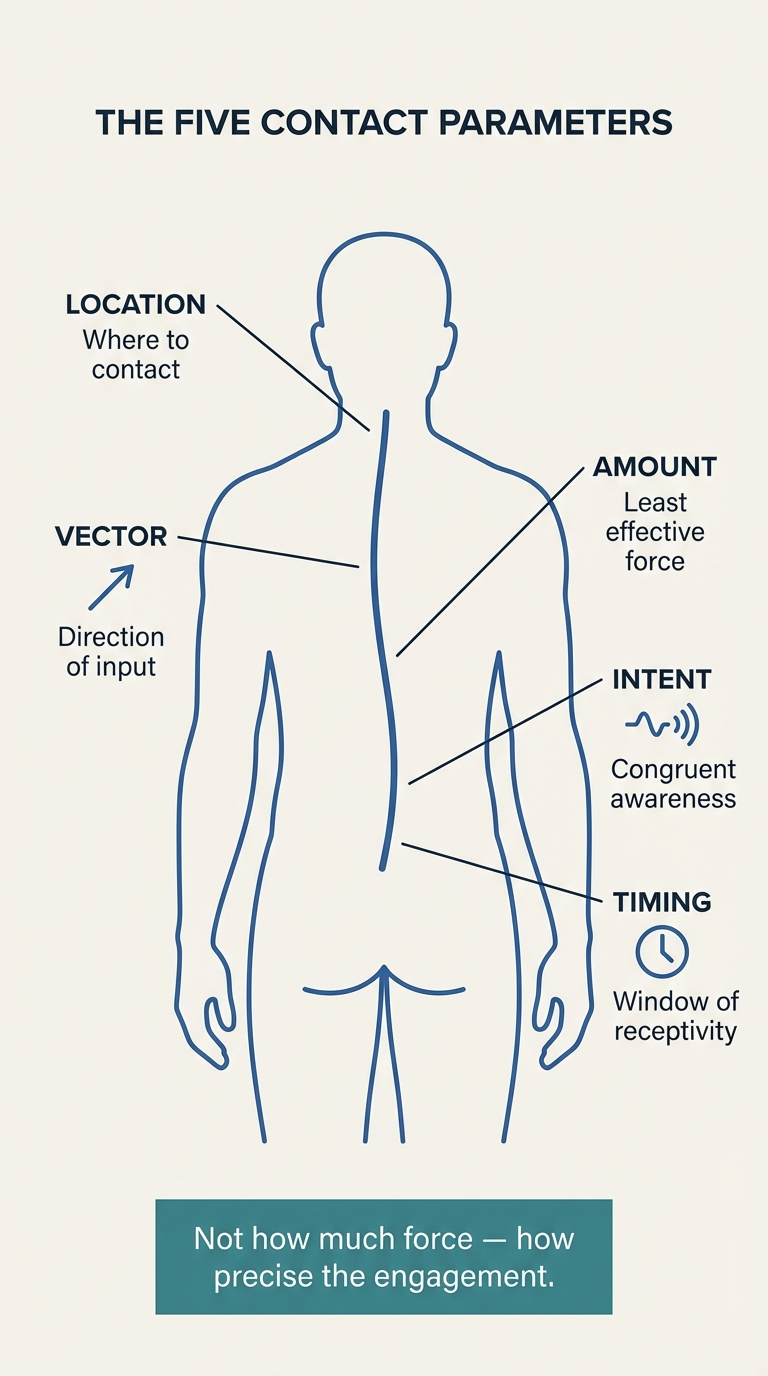
\includegraphics[width=0.85\textwidth]{15-contact-params-a-silhouette.png}
\caption{TTC Contact Parameters: Location, Vector, Amount, Intent}
\end{figure}
\FloatBarrier



TTC prioritizes global indicators for the signs of subluxation and the signs of subluxation reduction, rather than local segmental findings. We are not trying to find all the problems. We are trying to find the one place that is most ready and receptive to receive input.


\subsection{5.1 Global Tonal Indicators}

These indicators fall into three functional categories:


\subsubsection{Indicators Used to Measure Outcome Progression}

\textbf{A. Tissue Congestion}

Sign of stuck patterns due to chemical stress–induced subluxation.


\textbf{B. Breathing Patterns}

Wave of motion engaging from the sacrum to the occiput.


\textbf{C. Energy/Heat Radiation}

Breaks in continuity at transition zones identify likely access points and serve as markers for between-visit pattern analysis; persistent stuck patterns indicate subluxation.


\textbf{D. Postural Faults}

No longer able to properly adapt to forces of gravity in space.


\textbf{E. Muscle Patterns}

No longer appropriate sustained patterns of paraspinal muscle contraction. Most prevalent indication of an excessive response to perceived stress.


\subsubsection{Torsional vs Axial NeuroSpinal Tension — Indicators Used to Determine Line of Drive (LOD)}

\begin{itemize}
\item Foot flare (inversion/eversion)
\item Achilles Tension
\end{itemize}


\subsubsection{Indicators Used to Find the Best Window In}

\begin{itemize}
\item Functional Short leg
\item Ankle Pronation/Supination
\item Adduction Resistance
\item Derifield (Modified)
\item Cervical Syndrome (and associated findings)
\end{itemize}


\subsubsection{Verification Through System Balancing}

Within TTC, temporary system balancing (e.g., leg length equalization) serves as a working clinical indicator of receptivity, an internal operational signal used to guide contact decisions. Independent validation of this indicator as an objective diagnostic measure remains needed.


\subsection{5.2 Tonal Analysis and the Best Window In}

We assess global NeuroSpinal tone through tonal indicators in posture, breath, balance, energy, and tone — then locate the point of greatest receptivity through \textbf{tonal pressure testing} verified with the \textbf{neurological reflex of balanced legs}. These methods are used as one combined process, not separate tools. When the legs temporarily balance, TTC interprets this as a clinical indicator that the NeuroSpinal System is receptive to release in that specific vector and location at that moment.


\begin{pullquotebox}
"When the legs temporarily balance, TTC interprets this as a clinical indicator that the NeuroSpinal System is receptive to release in that specific vector and location at that moment."
\end{pullquotebox}


\subsection{5.3 Contact Parameters (Location, Vector, Amount, Intent)}

\textbf{Location:} Often at or near dural attachment "window" areas (craniocervical, sacro-coccygeal), but also along the course of identified aberrant tension in the NeuroSpinal System.


\textbf{Vector:} The Tonal Line of Drive—parallel to and opposite the direction of dural contraction, engaging the meningeal system in the direction of release.


\textbf{Amount:} Minimal. Enough to be perceived. Not enough to threaten.


\textbf{Intent:} Congruent with the physical input. The intent is to communicate with the body's intelligence through the physical matter of the nervous system.


TTC contact is a neurological communication. It is touch with vector and a congruent intent. It is given at the point of greatest receptivity. It is minimal, precise input. It cues the system's own adjustment process.


\begin{pullquotebox}
"TTC contact is a neurological communication. It is touch with vector and congruent intent. Given at the point of greatest receptivity. Minimal, precise input. It cues the system's own adjustment process."
\end{pullquotebox}

The model is now complete: mechanism, evidence, and method. TTC did not emerge from a vacuum. It is the next iteration in a long evolution of chiropractic thought — from compression-first to tension-aware to tone-first. Understanding that lineage explains why TTC's contributions are distinct, and why they are necessary.


\partbreak{Part VI. Historical Evolution: From Bone-on-Nerve to Tone-First}{The protocol is now in view. Before meeting the lineage that produced it, this section traces the intellectual arc — from compression-first models through tension-based models to the tonal framework TTC inherits and extends.}


\section{Part VI. From Bone-on-Nerve to Tone-First: Historical Evolution}

\begin{figure}[htbp]
\centering
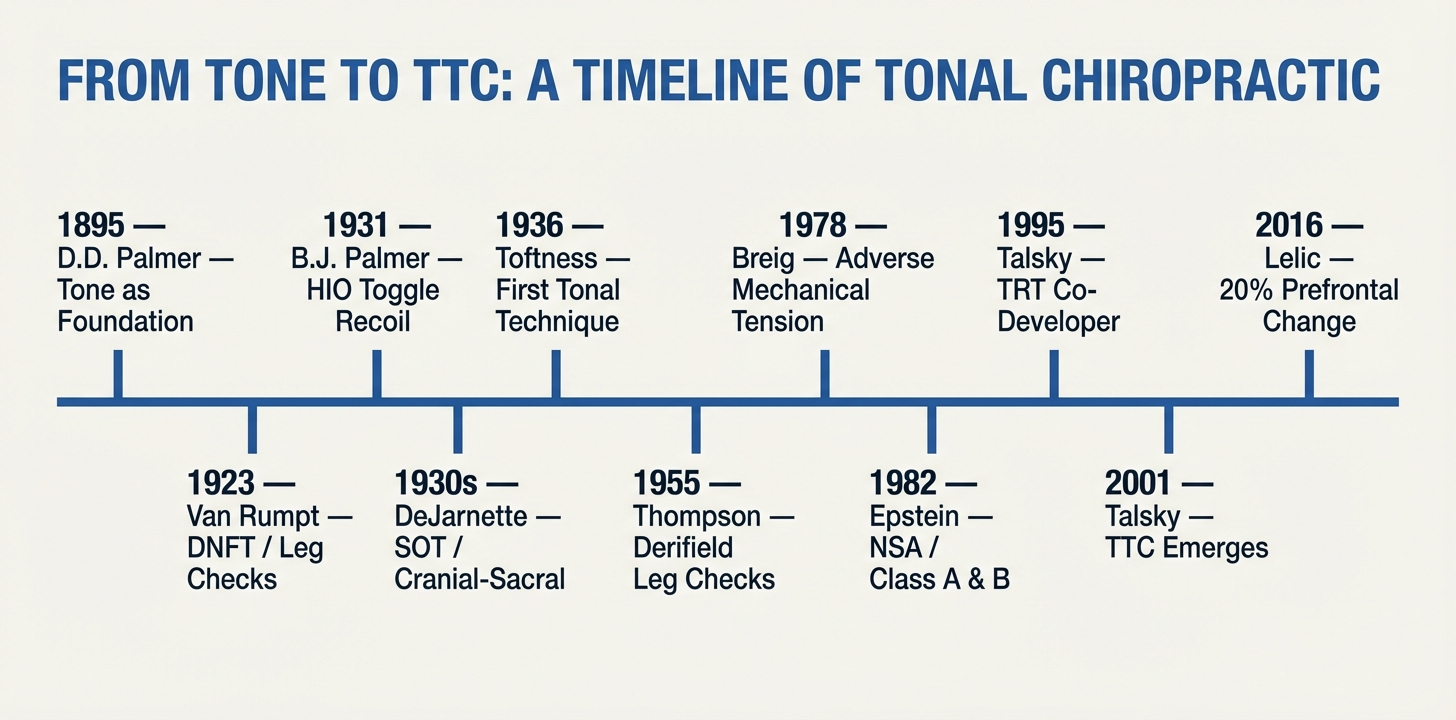
\includegraphics[width=0.85\textwidth]{07-timeline-a-horizontal.png}
\caption{Historical Timeline: From Bone-on-Nerve to Tone-First}
\end{figure}
\FloatBarrier




\subsection{6.1 The Traditional Subluxation Model: Compression First}

For most of chiropractic's history, subluxation was defined structurally, as a misalignment or fixation of spinal vertebrae producing neurological effects through mechanical compression or irritation. While this structural model helped establish chiropractic's early identity and produced meaningful clinical results, it entered the pathophysiological sequence at the level of vertebral compensation. Osseous models started with joint fixation and vertebral compensation, not recognizing that neurological interference begins upstream in the NeuroSpinal System (C-SMFU) with aberrant tension that drives those structural changes. They did not address the initiation of the subluxation process: the neurological interference in communication between brain and body that occurs first and foremost in the aberrant tension within the C-SMFU, initiating the cascade of dysfunction described in Part IV.


\subsection{6.2 The Shift from Compression to Tension-Based Interference}

Modern neuroscience increasingly challenges the long-held assumption that vertebral misalignment routinely causes neural interference through direct mechanical compression. Dr. Heidi Haavik's research has shown that interference more often stems from \textbf{tension, distortion, and altered afferent input}, not direct compression of nerve roots (Haavik \& Murphy, 2007).


Decades earlier, neurosurgeon \textbf{Dr. Alf Breig} documented that \textbf{Adverse Mechanical Tension (AMT)}, aberrant tension in the meningeal system and spinal cord, can disturb neural function even in the absence of vertebral displacement (Breig, 1978). His research revealed that the nervous system is vulnerable to stretch, torsion, and sustained tension, particularly when the dura and spinal cord are placed under aberrant mechanical load.


Within chiropractic, \textbf{Lowell Ward, D.C.} was the first to clinically apply Breig's AMT framework, integrating it into Spinal Column Stressology and conceptualizing the spine as a \textbf{"Spinal-Column-Pelvic-Meningeal-Unit"} — an anatomical description recognizing the cord-meningeal system as a unified structure (Ward, 1980). Building on Ward's anatomical awareness and Breig's biomechanics, \textbf{Donald Epstein, D.C.} in 1983 distinguished Class A (structural) subluxation from Class B (meningeal/facilitated), proposing that Class B originates not from vertebral misalignment but from tension within the cord-meningeal system itself (Epstein, 1996; see Section 6.4 for full discussion).


Together, their work challenged simple compression-only accounts and broadened the profession's attention toward tension, distortion, and altered afferent input:


\begin{center}
\begin{tabular}{lll}
\toprule
\rowcolor{primaryblue}
\textbf{\textsf{\color{white}Key Figure}} & \textbf{\textsf{\color{white}Core Finding}} & \textbf{\textsf{\color{white}Implication}} \\
\midrule
\rowcolor{lightbluebg!40}
\textbf{Alf Breig (1978)} & Demonstrated Adverse Mechanical Tension (AMT) in the meninges and spinal cord without vertebral displacement & Compression is not required for interference; tension itself is sufficient \\
\textbf{Lowell Ward (1980)} & First to clinically apply Breig's AMT within chiropractic; conceptualized the "Spinal-Column-Pelvic-Meningeal-Unit"; whole-spine stress patterns understood through meningeal tension & The cord-meningeal system recognized as a unified anatomical structure; Breig's neurosurgical insight becomes a chiropractic clinical framework \\
\rowcolor{lightbluebg!40}
\textbf{Donald Epstein (1982–1986)} & Coined Spinal Meningeal Functional Unit (SMFU); distinguished Class A (structural) from Class B (facilitated) subluxation; first to identify a class of subluxation originating in meningeal tension & Subluxation can originate in meningeal tension, not just vertebral misalignment; the cord-meningeal system is a unified clinical entity \\
\textbf{Heidi Haavik (2007)} & Altered sensorimotor integration traced to distorted afferent input, not nerve compression & Interference is primarily tonal and neurological, not compressive \\
\bottomrule
\end{tabular}
\end{center}


This shift from compression to tension represented a fundamental reconceptualization:


\begin{itemize}
\item \textbf{Compression model}: Bone → Nerve root → Dysfunction
\item \textbf{Tension model}: Stress → Meningeal tension → Altered neural signaling → Compensatory vertebral patterns
\end{itemize}

\begin{pullquotebox}
"The shift from compression to tension represented a fundamental reconceptualization: not bone on nerve root, but stress — meningeal tension — altered neural signaling — compensatory vertebral patterns."
\end{pullquotebox}


\subsection{6.3 Allostatic Load: A Physiological Model for Aberrant Tone}

TTC applies the allostatic load concept specifically to the NeuroSpinal System. The protective tightening described in Part I — and the dual distortions of misinformation and missing information it produces — represents allostatic load accumulating within the body's Primary Tone-Setter. When this load persists, the system can no longer recognize safety, and the protective pattern becomes maladaptive. Part IV details the full pathophysiology of why this pattern persists and how it is resolved.


\subsection{6.4 Facilitated Subluxation and Meningeal Models (Epstein)}

While tonal awareness in chiropractic practice predates Epstein, evident in the work of Toftness, Logan, and others who employed light-force, tone-aware methods decades earlier, \textbf{Donald Epstein, D.C.} made several interconnected contributions that transformed tonal chiropractic from a collection of individual techniques into a unified clinical framework.


\textbf{The SMFU concept.} Building on Ward's anatomical description of the "Spinal-Column-Pelvic-Meningeal-Unit" and Breig's biomechanical research on what Epstein would term \textbf{Adverse Mechanical Cord Tension (AMCT)}, adding "Cord" to Breig's broader AMT for greater anatomical specificity — and encouraged by chiropractor Thomas Faulkner to incorporate their work — Epstein coined the term \textbf{Spinal Meningeal Functional Unit (SMFU)} (Epstein, 1986). Where Ward had described the anatomy and Breig had demonstrated the mechanism, Epstein reframed the cord-meningeal system as a \textit{functional unit} with specific clinical implications: a dynamic, stress-responsive system whose tension state determines the organism's adaptive capacity.


\textbf{The Class A/B classification.} Epstein was the first to formally classify subluxation based on meningeal tension rather than vertebral misalignment. He distinguished between two classes:


\textbf{Class A (Structural Subluxation)}: A segmental distortion associated with compromise of intervertebral structures, most commonly produced by localized physical trauma. Traditional vertebral misalignment with associated fixation and local mechanical dysfunction.


\textbf{Class B (Facilitated Subluxation)}: Associated with lack of recovery from emotional, mental, or chemical stress and linked to Adverse Mechanical Cord Tension (AMCT). A tension-based state of the cord-meningeal system, often evident at dural "gateway" regions (craniocervical and sacro-coccygeal attachments). This is not primarily structural; it is a sustained protective contraction of the NeuroSpinal System that precedes and drives structural compensations. Epstein connected Class B to B.J. Palmer's earlier concepts of torqued meningeal occlusion and multiple cord pressures by tension, and related it functionally to Speransky's neurodystrophic processes.


\textbf{The integrated tonal analysis.} Before Epstein, techniques such as Toftness, Logan Basic, DNFT, SOT, Thompson, and Pierce-Stillwagon each operated in isolation, detecting different aspects of spinal tension through their own indicators and protocols. Epstein's insight was that these techniques were all detecting facets of the same underlying cord-meningeal phenomenon. He synthesized their assessment methods — paraspinal thermal patterns, leg checks, palpation, reflex indicators — into a single, technique-agnostic analysis framework capable of differentiating Class A from Class B subluxation and guiding appropriate intervention.


\textbf{Wave dynamics.} Epstein recognized that gentle, low-force contacts at dural gateway areas could cue reorganizational responses, including the emergence of two distinctive wave phenomena: the \textbf{respiratory wave} (a breath-driven oscillation reflecting enhanced somatic awareness) and the \textbf{somatopsychic wave} (a propagating pattern of movement reflecting deeper nervous system reorganization and mind-body integration). First clinically demonstrated in 1987, these wave dynamics represent observable markers of the nervous system's reorganizational capacity. Subsequent research at the University of Southern California characterized the Network Spinal Wave as a central pattern generator — the first identified in the spinal cord unrelated to locomotion or respiration (Senzon, Epstein, \& Lemberger, 2016).


\textbf{This was the first professional articulation within chiropractic of the initiatory neurophysiological step in the process of subluxation and subluxation reduction, specifically for what Epstein termed Class B (facilitated) subluxation. His SMFU framework, Class A/B classification, integrated tonal analysis, and wave dynamics research represent foundational contributions upon which all subsequent tonal models build.}


\begin{pullquotebox}
"This was the first professional articulation within chiropractic of the initiatory neurophysiological step in the process of subluxation and subluxation reduction, specifically for what Epstein termed Class B (facilitated) subluxation."
\end{pullquotebox}

Epstein's model, however, remained primarily clinical and observational — he described and demonstrated the phenomenon but did not address the underlying biology. The mechanobiological questions are addressed by TTC in Part IV.


\textbf{A note on terminology.} Breig used the term \textbf{Adverse Mechanical Tension (AMT)} to describe aberrant tension in the meningeal system and spinal cord. Epstein refined this to \textbf{Adverse Mechanical Cord Tension (AMCT)}, adding "Cord" for greater anatomical specificity. TTC adopts the term \textbf{aberrant NeuroSpinal tension} throughout this paper, reflecting the clinical observation that dural tension frequently manifests at the occiput, sphenoid, and zygoma — areas that extend well beyond what "cord" alone captures. The phenomenon is the same; the terminology reflects each model's expanding scope of anatomical engagement.


TTC builds directly on Epstein's insight and extends it in two directions — \textbf{science and application}:


\textbf{The science.} TTC proposes that meningeal involvement is present in \textbf{all} subluxation, including Class A. Even where physical trauma genuinely displaces a joint (Class A), the sustained dyskinesia that follows is associated with meningeal contracture. The trauma moves the bone, but the meningeal bracing that locks around it is what prevents resolution. Part IV presents the full mechanobiological model explaining why this contraction persists and why specific input is required to facilitate release.


\textbf{The application.} Where Epstein's clinical model contacts segments associated with peaceful states at gateway regions to cue reorganizational wave responses, TTC takes a different methodological path. TTC relies on mandatory tonal pressure testing with leg balancing to identify the exact location, vector, and timing of every contact — the system must confirm receptivity before input is delivered. The contact vector is then derived directly from the meningeal contraction itself: parallel to and opposite the direction of dural contraction, engaging in the direction of release. This contraction-specific vector — the Tonal Line of Drive — is unique to TTC and follows directly from the mechanobiology: if the meninges hold tension in a specific direction, the input must engage that tension in the direction of release, not simply at a gateway region. The result is a method that is more reliant on real-time neurological verification (pressure testing) and more precisely oriented toward the specific meningeal contraction pattern than any prior tonal approach.


By addressing this meningeal contracture directly, the body can begin resolving the subluxation on its own. This means there is a primary NeuroSpinal tone pattern that must be addressed before vertebral work will have lasting effect, regardless of whether the subluxation originated structurally or through facilitation. \textbf{(For acknowledgment of Network Spinal's foundational contributions and TTC's distinct methodological approach, see Section 7.4.)}


\subsection{6.5 From Segmental to Systems Thinking}

The historical trajectory outlined above, from compression to tension to tone, reflects a broader shift in how chiropractic understands the body: from a segmental, joint-by-joint model to a systems-based model of tone regulation. Modern understanding of neuroplasticity, biotensegrity, and complex adaptive systems supports this evolution. The spine is not a column of independent segments to be corrected one at a time; it is a tensionally integrated whole whose behavior emerges from the global state of its Primary Tone-Setter, the NeuroSpinal System. TTC represents the clinical application of this systems-level understanding: working with the organizing principle of the whole rather than the compensations of its parts.


\begin{pullquotebox}
"The spine is not a column of independent segments to be corrected one at a time; it is a tensionally integrated whole whose behavior emerges from the global state of its Primary Tone-Setter."
\end{pullquotebox}

The conceptual evolution from compression to tension to tone establishes \textit{what} changed and \textit{why}. Part VII traces the practitioners who drove that evolution — the specific individuals and techniques whose contributions form TTC's direct lineage.


\partbreak{Part VII. Historical Lineage and Positioning}{TTC did not appear from nowhere. This section traces the practitioners who built the conceptual and clinical infrastructure TTC inherits — and maps TTC's relationship to the approaches that most closely preceded it.}

\begin{figure}[htbp]
\centering
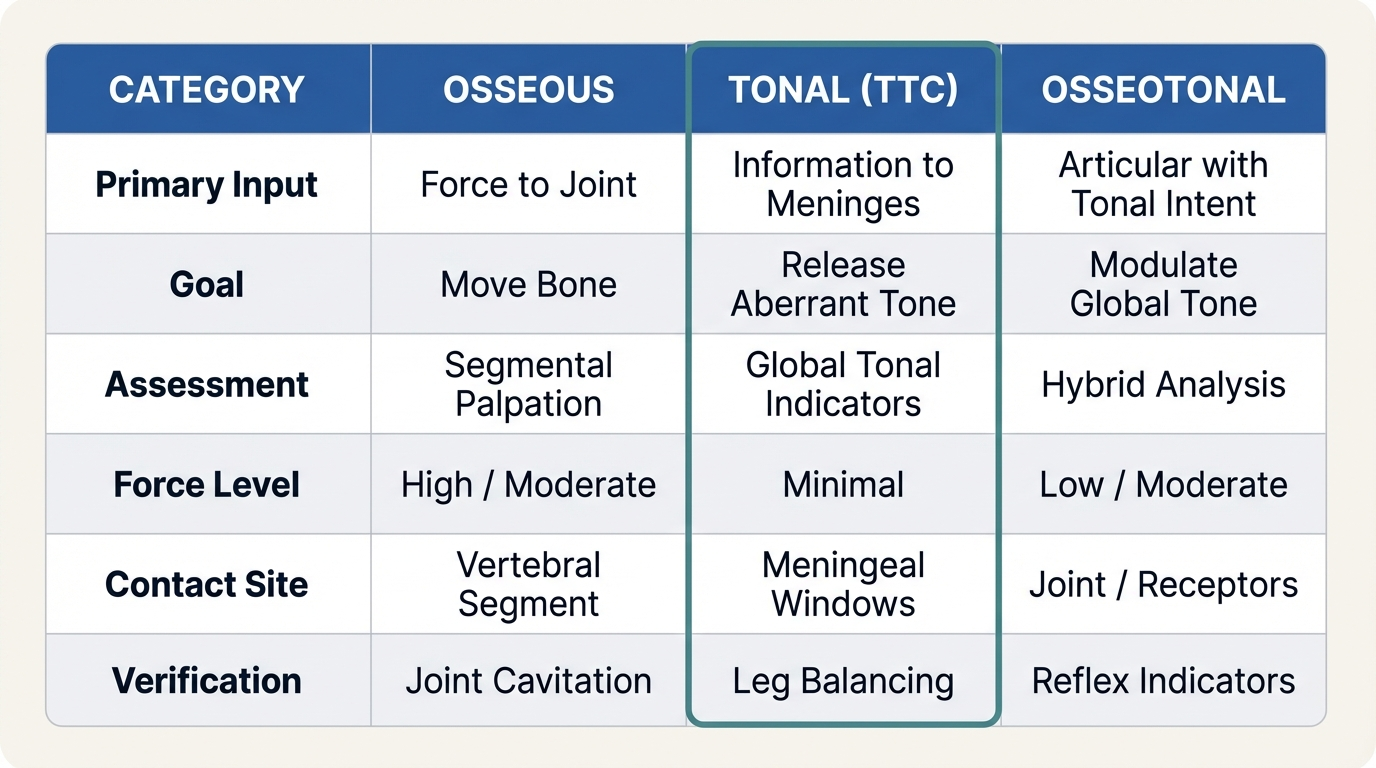
\includegraphics[width=0.85\textwidth]{06-technique-table-a-four-column.png}
\caption{Technique Comparison: Osseous, OsseoTonal, Tonal, Tonal Energetics}
\end{figure}
\FloatBarrier


\section{Part VII. Historical Lineage and Positioning}



\subsection{7.1 Tonal Pioneers}

The evolution from structural to tonal models was gradual, built on the insights of many innovators:


\textbf{Daniel David Palmer, D.C. (1895)}: Founded chiropractic in Davenport, Iowa, establishing tone as chiropractic's foundational principle. In \textit{The Chiropractor's Adjuster} (1910), Palmer wrote: \textit{"Life is an expression of tone; the cause of disease is any variation in tone."} His philosophy of Innate Intelligence and tone-based interference laid the vitalistic foundation for all subsequent tonal approaches in chiropractic.


\textbf{Richard Van Rumpt, D.C. (1923–1930s)}: Created \textbf{Directional Non-Force Technique (DNFT)}, making widespread use of leg checks and reflex indicators to identify the optimum point and direction of correction. Van Rumpt is credited with discovering in 1923 that a very specific light-force thrust could produce the same corrective response traditionally attributed to high-force manipulation, perfecting the reactive leg reflex in the 1930s. DNFT demonstrated that force was not necessary for neurological change; precise information was more important. Van Rumpt is credited as the original developer of the "reactive leg reflex."


\begin{pullquotebox}
"Van Rumpt is credited with discovering in 1923 that a very specific light-force thrust could produce the same corrective response traditionally attributed to high-force manipulation. Force was not necessary for neurological change; precise information was more important."
\end{pullquotebox}

\textbf{Major Bertrand DeJarnette, D.C. (1930s–1940s)}: Developed \textbf{Sacro-Occipital Technique (SOT)}, which introduced the concept of using indicators to assess the body's organizational state and emphasized cranial-sacral relationships and the role of the meninges in coordinating spinal mechanics.


\textbf{B.J. Palmer, D.C. (1931)}: Developed the \textbf{HIO (Hole-In-One) Toggle Recoil} upper cervical technique, recognizing that specific cranio-cervical contacts could influence global function through articular engagement of the upper cervical spine.


\textbf{Hugh B. Logan, D.C. (1931)}: Developed \textbf{Logan Basic Technique (LBT)}, presenting his "Universal Health-Basic Technique" which focused on the sacrum as the base of the spine. Logan reasoned that if the sacrum was subluxated, it would affect the stability of the entire spine. The technique uses light force contact on the sacrotuberous ligament, demonstrating early tonal awareness in addressing spinal mechanics through sustained, gentle pressure.


\textbf{Irwing N. Toftness, D.C. (1936–1950s)}: Developed \textbf{Toftness Technique}, widely regarded as the first completely tonal chiropractic technique. Dr. Toftness is widely remembered within the profession for consistently winning pre- and post-x-ray competitions for the reduction in scoliosis hosted at Logan University, demonstrating the clinical effectiveness of his tonal approach.


\textbf{Dr. John F. Grostic, Sr., D.C. (1941–1964)}: Working with Dr. Ralph R. Gregory starting in 1941, Dr. Grostic developed the \textbf{dentate ligament cord distortion hypothesis} and the \textbf{Grostic Technique}, a precise, low-force upper cervical method recognizing that specific cranio-cervical contacts could influence global tone via structural articular engagement of the upper cervical spine and dentate ligament tension patterns. After Grostic's death in 1964, Dr. Gregory formed the National Upper Cervical Chiropractic Association (NUCCA) in 1966.


\textbf{J. Clay Thompson, D.C. (1950s)}: Expanded on leg checks and indicators within a more structural model (\textbf{Thompson Technique}), using Derifield leg checks (which originated from DNFT's reflex indicator foundation) and developing them into the Thompson-Derifield analysis system combined with his patented drop-table system (1955).


\textbf{Alf Breig, M.D., Ph.D. (1960–1978)}: Swedish neurosurgeon whose pioneering research on \textbf{Adverse Mechanical Tension in the Central Nervous System} (1978) demonstrated that tension in the meningeal system and spinal cord can disturb neural function even in the absence of vertebral displacement. His work reframed the conversation from compression-based to tension-based models of neurological interference, providing scientific foundation for tonal approaches.


\textbf{Lowell Ward, D.C. (1970s–1980s)}: Developer of \textbf{Spinal Column Stressology (SCS)} and author of \textit{The Dynamics of Spinal Stress}. Dr. Ward conceptualized the spine as a \textbf{"Spinal-Column-Pelvic-Meningeal-Unit,"} recognizing the cord-meningeal system as a unified anatomical structure and describing subluxation as occurring within this integrated system rather than at isolated segments. Working with aerospace engineer Fulkerson and integrating Breig's biomechanics, Ward emphasized whole-spine stress patterns revealed through seated and standing full-spine x-rays. His anatomical framework directly influenced Epstein's subsequent Spinal Meningeal Functional Unit concept.


\textbf{Donald Epstein, D.C. (1982)}: Created \textbf{Network Chiropractic} (now \textbf{Network Spinal}). Coined the \textbf{Spinal Meningeal Functional Unit (SMFU)} and was the first to formally articulate the cord-meningeal system as the initiating site of subluxation. His SMFU framework, Class A/B subluxation classification, technique synthesis, and wave dynamics represent foundational contributions upon which all subsequent tonal models build, including TTC. \textbf{(See Part VI, Section 6.4 for full treatment of Epstein's contributions; Section 7.4 for TTC's relationship to this work.)}


\textbf{Marvin Talsky, D.C. (1995–2001)}: Co-developed \textbf{Torque Release Technique (TRT)} in 1995 with Dr. Jay Holder, who invented the Integrator instrument. Talsky developed and structured the Torque Release Model after 30 years of continuous practice. Talsky's work emphasized \textbf{direct engagement with the NeuroSpinal system} and the concept that the body could self-adjust when given the right informational input. Talsky continued to refine a more direct, non-articular, NeuroSpinal engagement, which evolved into \textbf{Talsky Tonal Chiropractic} in 2001.


\textbf{Heidi Haavik, D.C., Ph.D. (2007–present)}: New Zealand chiropractor and neurophysiologist whose research demonstrated that neural interference more often stems from \textbf{tension, distortion, and altered afferent input} rather than direct compression of nerve roots. Her research has found evidence of measurable changes in brain function following chiropractic adjustments. A brain source localization study (Lelic et al., 2016) estimated changes of nearly 20\% in prefrontal cortex processing following adjustment of dysfunctional spinal segments, though the authors note that further research with larger samples is needed to confirm these preliminary findings. Her work has advanced understanding of neuroplasticity and sensorimotor integration in the context of chiropractic care. Haavik's research protocols employed articular spinal manipulation, not non-articular tonal contacts; applying these findings to TTC specifically remains a research priority (see Part III). Dr. Haavik's work provided supportive evidence that spinal manipulation produces measurable neurophysiologic effects, lending credibility to tension-based models of subluxation.


\textbf{Simon Senzon, D.C. (2010s)}: Through peer-reviewed articles and historical analysis, Dr. Senzon contributed to the philosophical coherence of tonal chiropractic, applying \textbf{Integral Theory} to bridge modern scientific frameworks with the vitalistic heritage of chiropractic.


\subsubsection{Summary: Foundational Contributions to Tonal Chiropractic}


\begin{center}
\begin{tabular}{ll}
\toprule
\rowcolor{primaryblue}
\textbf{\textsf{\color{white}Era / Technique}} & \textbf{\textsf{\color{white}Tonal Contribution}} \\
\midrule
\rowcolor{lightbluebg!40}
\textbf{D.D. Palmer (1895)} & Established tone as chiropractic's foundational principle \\
\textbf{Van Rumpt / DNFT (1923)} & Introduced pressure testing and leg checks as reflex indicators \\
\rowcolor{lightbluebg!40}
\textbf{DeJarnette / SOT (1930s)} & Cranial-sacral relationships; meningeal role in spinal mechanics \\
\textbf{Logan Basic (1931)} & Low-force sacral contacts to balance postural tone \\
\rowcolor{lightbluebg!40}
\textbf{B.J. Palmer / HIO (1931)} & Upper cervical contacts influencing global function \\
\textbf{Grostic (1941)} & Dentate-ligament cord distortion hypothesis \\
\rowcolor{lightbluebg!40}
\textbf{Toftness (1936)} & First completely tonal chiropractic technique \\
\textbf{Thompson (1955)} & Leg checks as neurological tone indicators \\
\rowcolor{lightbluebg!40}
\textbf{Breig (1978)} & Adverse Mechanical Tension: tension-based interference without vertebral displacement \\
\textbf{Ward / SCS (1980)} & "Spinal-Column-Pelvic-Meningeal-Unit"; spine as whole-system dynamic stress pattern \\
\rowcolor{lightbluebg!40}
\textbf{Epstein / NSA (1982)} & Coined SMFU; distinguished Class A (structural) from Class B (facilitated/meningeal); wave dynamics; tonal analysis synthesis \\
\textbf{Talsky / TRT → TTC (1995–2001)} & Direct NeuroSpinal engagement; pure tonal chiropractic \\
\rowcolor{lightbluebg!40}
\textbf{Haavik (2007)} & Neurophysiologic evidence supporting tension-based subluxation models \\
\bottomrule
\end{tabular}
\end{center}


\subsection{7.2 The Emergence of OsseoTonal Models}

As tonal methods matured, a new category emerged: \textbf{OsseoTonal}, approaches that retain tonal awareness of the NeuroSpinal System but choose to engage it through joint articulations or joint-space mechanoreceptors.


Any osseous (structural) technique that includes awareness of and reverence for the NeuroSpinal System and incorporates at least some aspect of tonal awareness and intent, both in the analysis for and in the application of osseous adjustments, can be considered OsseoTonal. These approaches demonstrate that \textbf{tonal awareness can enhance traditional structural approaches}, allowing practitioners to work with both structural mechanics and global tone simultaneously.


\begin{center}
\begin{tabular}{ll}
\toprule
\rowcolor{primaryblue}
\textbf{\textsf{\color{white}OsseoTonal Technique}} & \textbf{\textsf{\color{white}Distinguishing Features}} \\
\midrule
\rowcolor{lightbluebg!40}
\textbf{Torque Release Technique (TRT, 1995)} & Instrument-assisted input with pressure testing and leg checks; strong tonal intent \\
\textbf{MC2 (1996)} & Balances tone via upper cervical contacts and reflex-based indicators \\
\rowcolor{lightbluebg!40}
\textbf{Bio-Geometric Integration (BGI, 1995)} & Adjustments guided by biotensegrity and wave propagation \\
\textbf{Mastery Love Service (MLS)} & Prioritizes tone, presence, and honoring Innate Intelligence through intentional osseous adjustments \\
\rowcolor{lightbluebg!40}
\textbf{Tonal Integrative Correction (TIC)} & Combines meningeal, structural, and tonal indicators with harmonic resonance modeling \\
\textbf{Kairos Training Culture (KTC)} & Adjusting mastery, breath, biomechanics, and energetic flow with tonal awareness \\
\rowcolor{lightbluebg!40}
\textbf{Syntropy Chiropractic Training} & Peak adjusting performance with tonal structure and flow-state awareness \\
\textbf{Pneuma Chiropractic} & Integrates neural and vibrational awareness into structural adjustments \\
\bottomrule
\end{tabular}
\end{center}


\subsection{7.3 The Evolution from Torque Release Technique to Talsky Tonal Chiropractic}

\textbf{Talsky's Tonal Lineage:}

Dr. Marvin Talsky's development of tonal approaches drew from direct study with many of the key contributors to tonal chiropractic. Prior to his five years of study under Dr. Donald Epstein, Talsky had already studied DNFT, Toftness, and Logan techniques, worked with Dr. Clay Thompson for 10 years, and practiced with the Activator for many years. This extensive foundation in techniques that have contributed to tonal chiropractic provided Dr. Talsky with deep understanding of the principles and protocols underlying tonal analysis and application.


Epstein's synthesis of pre-existing indicators into a unified tonal framework (see Part VI, Section 6.4), combined with theoretical frameworks from Breig, Ward, Speransky, and Korr (facilitation hypothesis), was the foundation Talsky built on during his five years of study, integrating these insights with his prior decade-plus of experience in tonal methods.


\textbf{The TRT Foundation:}

Building on this extensive background, Dr. Talsky co-developed and structured the \textbf{Torque Release Technique (TRT)} protocol in 1995 with Dr. Jay Holder, who invented the Integrator instrument. Talsky's structuring of TRT represented an OsseoTonal approach: vectors were originally oriented osseously with tonal awareness and intent, engaging joint articulations to influence the NeuroSpinal System. TRT combined the precision of instrumentation with tonal indicators and leg check verification, demonstrating that tonal awareness could enhance structural engagement.


\textbf{The Evolution to TTC:}

Through continued refinement and clinical observation, Talsky recognized that even more direct engagement with the NeuroSpinal System was possible. Beginning in 2001, \textbf{Talsky Tonal Chiropractic} emerged as a completely tonal model and technique, distinguished by contact points and vectors oriented toward NeuroSpinal release rather than oriented around joint articulations. TTC moved beyond the OsseoTonal model to work exclusively through tonal mechanisms: non-articular, non-osseous, with vectors strictly parallel to aberrant tension in the meningeal-dural continuum.


\textbf{TTC is the evolution of TRT} and continues to evolve to this day as new discoveries and refinements emerge. Where TRT engaged tone through osseous contacts, TTC engages the NeuroSpinal System directly through its own structure: the Cranio-Spinal Meningeal Functional Unit (C-SMFU).


\subsection{7.4 TTC and Network Spinal: Shared Foundations, Distinct Approaches}

\textbf{Acknowledging Network Spinal's foundational contributions:}

Without Epstein's foundational insight — that a class of subluxation originates in cord-meningeal tension — TTC as it exists today would not be possible (see Part VI, Section 6.4 for the full account of these contributions). Both TTC and Network Spinal recognize key gateway zones at craniocervical and sacro-coccygeal dural attachments and use indicators and low-force contacts to cue whole-system responses. TTC's debt to this body of work is explicit and gratefully acknowledged.


\textbf{Where TTC distinguishes itself as working exclusively through tonal mechanisms:}

TTC maintains exclusive focus on \textbf{physical inputs to physical nervous system structures}. TTC does not make the network wave a clinical aim, does not require wave entrainment, and does not intentionally work with energetic facilitation, transformational energetic processes, or reorganizational healing frameworks that extend beyond the mechanobiological effects of precisely applied tension and timing. Network Spinal is appropriately categorized as incorporating aspects of \textbf{Tonal Energetics}, a valuable approach that explicitly integrates energetic facilitation with tonal awareness. TTC remains within \textbf{Tonal Chiropractic}: directional corrective intent communicated through touch to a system whose inherent drive is to resolve and reorganize.


\textbf{TTC's unique contributions:}


\begin{enumerate}
\item \textbf{Mechanobiological model of meningeal contractility}: To the authors' knowledge, TTC provides the first mechanobiological explanation within chiropractic for meningeal contraction and persistence (see Part IV for the full model). Where Epstein's framework identified the clinical phenomenon, TTC supplies the underlying science. This model also explains why all subluxation — not only Class B — involves meningeal contracture.
\end{enumerate}

\begin{enumerate}
\item \textbf{Dural contraction-specific vectors (the Tonal Line of Drive)}: Where osseous methods direct force into joint spaces and Network Spinal contacts gateway regions, TTC derives its contact vector from the meningeal contraction itself — the Tonal Line of Drive described in Part V. This vector is unique to TTC.
\end{enumerate}

\begin{enumerate}
\item \textbf{Mandatory tonal pressure testing with leg balancing}: Every contact is verified through real-time neurological indicators before input is delivered. The system must show temporary balancing in response to a directional pressure test, confirming that the specific location, vector, and timing are correct for that contact at that moment. This makes TTC more reliant on real-time neurological verification than any prior tonal approach — the practitioner does not proceed without the system's confirmation.
\end{enumerate}

\begin{enumerate}
\item \textbf{Non-articular engagement of the NeuroSpinal System}: Strictly meningeal and dural contacts, not through joint spaces or articular mechanoreceptors
\end{enumerate}

\begin{enumerate}
\item \textbf{Model-first approach}: TTC functions as both a conceptual framework and model (applicable to inform any technique) and a complete standalone technique
\end{enumerate}

\begin{enumerate}
\item \textbf{Explicit Physical-only intent}: Congruent intent to communicate with the body's organizing intelligence through the physical matter of the nervous system, without any intentional energetic therapeutics.
\end{enumerate}

Where Epstein opened the door, TTC walks through it — with the science, the clinical method, and the real-time verification described throughout this paper.


\begin{pullquotebox}
"Without Epstein's foundational insight — that a class of subluxation originates in cord-meningeal tension — TTC as it exists today would not be possible. Where Epstein opened the door, TTC walks through it — with the science, the clinical method, and the real-time verification."
\end{pullquotebox}


\subsection{7.5 The Technique Landscape}

\textbf{Osseous approaches} use enough force to move a bone via an articular input.


\textbf{Tonal approaches} engage the NeuroSpinal System as a tensional organ first, using non-articular inputs guided by global indicators and verified by system balancing.


\textbf{OsseoTonal approaches} retain tonal awareness of the NeuroSpinal System but engage it through joint articulations or by stimulating mechanoreceptors within joint spaces with the intent to modulate global tone.


\textbf{Tonal Energetics} employ tonal awareness with explicit energetic facilitation, including work with transformational energetic processes. TTC distinguishes itself by maintaining focus on physical inputs to physical nervous system structures, guided by focused intent and without the use of any intentional energetic therapeutics.


With the model, the mechanism, the method, and the lineage established, the practitioner faces a practical question: what should patients expect, and what ethical commitments govern TTC practice?


\partbreak{Part VIII. Clinical Expectations and Ethics}{History and science are now behind us. This section turns toward the person in the room — what the practitioner aims for, how progress is recognized, and how TTC's principles translate across different clinical approaches.}


\section{Part VIII. Clinical Expectations And Ethics}


The clinical ethic of TTC is precision and responsibility with a reverence for the body's organizing intelligence.


Trajectory we aim for: more optimally distributed tone, improved breath and balance, increased resilience to stressors, better recovery after stressors, and a subjective sense of ease and integration, all signs of the reduction of subluxation. This approach supports ongoing optimization through care, evolving toward greater adaptability, regulation, and wholeness.


By releasing protective tone and restoring clear informational flow, TTC facilitates an adaptive reorganization process:


\begin{itemize}
\item Expanding the body's \textbf{decision space} (capacity for adaptive choice)
\item Enhancing the variability and fidelity of sensory input
\item Allowing more precise motor output and physiological regulation
\end{itemize}

This is what people experience as ongoing improvement in function and adaptability. We are not just getting them to maintenance. We are helping them keep evolving in adaptability, coherence, and wholeness.


\begin{pullquotebox}
"We are not just getting people to maintenance. We are helping them keep evolving in adaptability, coherence, and wholeness."
\end{pullquotebox}


\subsection{For the Practitioner: Integrating TTC Principles}

\textbf{If you practice osseous techniques:} Use global tonal indicators to inform your segmental analysis. Ask: "What is the NeuroSpinal tone pattern driving this fixation?" Address both cause and effect.


\textbf{If you practice tonal techniques:} Consider whether your vectors engage the meningeal-dural continuum directly, or influence it indirectly through articular mechanoreceptors. Refine toward precision and receptivity.


\textbf{For all:} The shift from "finding fixations" to "finding receptivity" is not technique; it's paradigm. It changes how you see, how you listen, and how you adjust.


\begin{pullquotebox}
"The shift from 'finding fixations' to 'finding receptivity' is not technique; it's paradigm. It changes how you see, how you listen, and how you adjust."
\end{pullquotebox}


\section{Part IX. TTC Glossary}


\textbf{Adaptive Reorganization}: In TTC, the process by which the body integrates new information to create a higher level of coordination, adaptability, and coherence.


\textbf{Allostatic Load}: The physiological cost of chronic stress adaptation. In TTC, prolonged elevated baseline tone within the NeuroSpinal System increases susceptibility to dysfunction and represents the sustained energetic burden of the protective meningeal response.


\textbf{Aberrant NeuroSpinal Tension}: TTC's term for the state of sustained, stress-mediated tension in the meningeal system that disturbs neural function. Historically, Breig (1978) described this as \textbf{Adverse Mechanical Tension (AMT)}; Epstein refined it to \textbf{Adverse Mechanical Cord Tension (AMCT)}, adding "Cord" for anatomical specificity. TTC adopts "aberrant NeuroSpinal tension" because dural tension frequently manifests at the occiput, sphenoid, and zygoma — areas beyond what "cord" alone captures (see Part VI, Section 6.4 for full terminology note). In the TTC model, aberrant NeuroSpinal tension develops from protective meningeal contraction in response to actual or perceived threat. The initial response involves contraction of existing myofibroblasts. Under sustained load, additional fibroblasts convert to myofibroblasts via TGF-β1 signaling, a mechanism demonstrated in meningeal tissue under pathological conditions (Dorrier et al., 2021), progressively deepening the tension and increasing subluxation severity through time. This aberrant tension persists beyond the stressor until sufficient safety signals permit release.


\textbf{Best Window In}: In TTC, a spatiotemporal opportunity when system receptivity is highest to a minimal, well-oriented input. The most receptive and responsive area of the NeuroSpinal System for a given practitioner at a given time, determined through tonal indicators and verified by a temporary complete leg balancing following a tonal pressure test.


\textbf{Congruent Intent}: In TTC, alignment of focused intent and physical action; the coherence between what the chiropractor intends and what the hands communicate. The intent to communicate with the intelligence of the body through the physical matter of the nervous system.


\textbf{Cranio-Spinal Meningeal Functional Unit (C-SMFU)}: TTC's extension of Donald Epstein's Spinal Meningeal Functional Unit (SMFU), emphasizing the cranial pole alongside spinal and sacral attachments. See NeuroSpinal System.


\textbf{Facilitated Subluxation (Epstein, Class B)}: A tension-based state of the cord-meningeal system, often evident at dural gateway regions (synonymous with windows in TTC), that can be addressed with gentle, low-force contacts which cue reorganizational responses. Distinct from structural (Class A) subluxation. Epstein's articulation of this concept was the first professional articulation within chiropractic of the initiatory neurophysiological step in subluxation. TTC extends this insight to propose that meningeal involvement is present in all subluxation, including Class A.


\textbf{Least amount of the most effective input}: In TTC, the application ethic guiding contacts in amplitude and quantity, a critical tonal protocol. Enough to be heard by the system, not enough to interfere with the system's own corrective process.


\textbf{NeuroSpinal System}: In TTC, the integrated system of the brain, spinal cord, pia mater (including the dentate ligament), arachnoid space (including cerebrospinal fluid), dura mater, and the connective tissue attachments to the movable bony structures of the cranium and spine. The outer dural sheath extends continuously into the surrounding fascial network, positioning the NeuroSpinal System as a primary tone-setter for the body's fascia as well. Synonymous with Cranio-Spinal Meningeal Functional Unit (C-SMFU). TTC defines this as the foundational physical system that sets the tone through which Innate Intelligence coordinates the body's actions.


\textbf{NeuroSpinal Subluxation}: In TTC, aberrant global tone within the NeuroSpinal System that degrades adaptability and regulation. TTC proposes this as the initiatory mechanism that precedes and drives the structural changes observed in the Vertebral Subluxation Complex.


\textbf{Osseous Adjustment}: An adjustment that directly engages joint articulations or vertebral segments to change structure and joint mechanics.


\textbf{Tonal Adjustment}: In TTC, an adjustment that engages the NeuroSpinal System through tone via directional informational input with congruent intent, non-articular and low force, communicating corrective intent through touch to an intelligent system that wants to correct.


\textbf{OsseoTonal Adjustment}: An adjustment that retains tonal awareness of the NeuroSpinal System while engaging it through joint articulations or by stimulating mechanoreceptors within joint spaces to influence global tone.


\textbf{Primary Tone-Setter}: TTC defines the Primary Tone-Setter as the NeuroSpinal System in its role as the foundational regulator of global tone; when it holds aberrant tension, all downstream systems compensate.


\textbf{Tonal Pressure Testing}: In TTC, a diagnostic method used to determine where the NeuroSpinal System can receive and integrate input without resistance or overwhelm. Applied through gentle directional pressure at potential contact points, verified by the neurological reflex of balanced legs.


\textbf{Tone}: In TTC, the baseline state of tension, coherence, and responsiveness within the nervous system and its connective tissue envelope. Within the chiropractic philosophical tradition, tone is the mechanism through which Universal Intelligence manifests and maintains the physical universe and the medium through which Innate Intelligence coordinates all actions. Tone is intelligence in motion.


\textbf{Tonal Line of Drive / Vector of release}: In TTC, the contact vector derived from the meningeal contraction itself—delivered parallel to and opposite the direction of dural contraction, engaging the dura or its direct extension in the direction of release. This contraction-specific vector—parallel to the tension and in the direction of release—is unique to TTC.


\section{Part X. Epilogue: The Self-Tuning Guitar}

\begin{figure}[htbp]
\centering
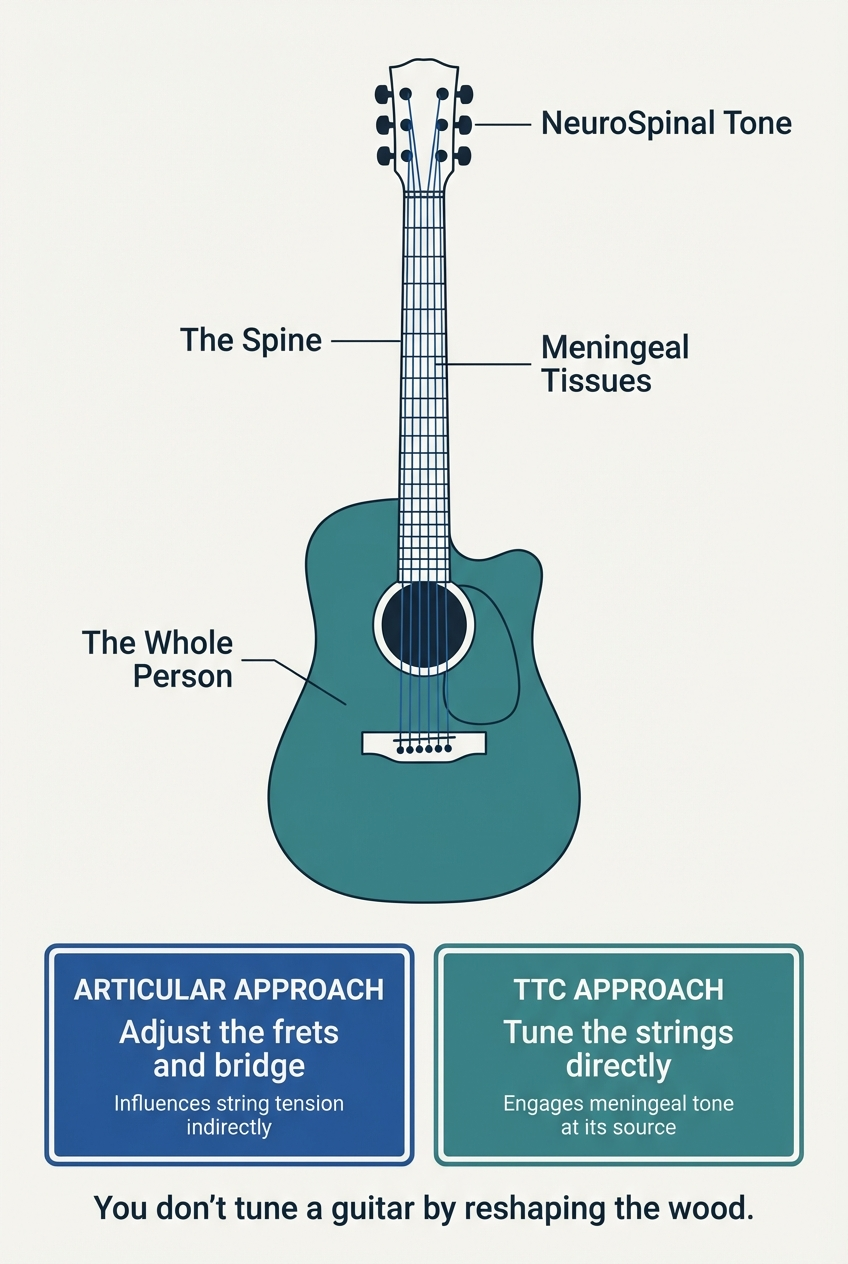
\includegraphics[width=0.85\textwidth]{12-guitar-a-instrument.png}
\caption{The Self-Tuning Guitar: A Metaphor for TTC}
\end{figure}
\FloatBarrier



Imagine the NeuroSpinal System as a self-tuning guitar, one equipped with advanced AI, sensors, and precision mechanics that can tune itself better than any human ever could. As it's played, it continuously adjusts, achieving perfect resonance. But sometimes the tuning mechanism physically gets stuck. The best thing a human can do is nudge the tuner gently in the right direction and let the intelligence of the system take over.


That's the essence of Talsky Tonal Chiropractic: finding the best window into the NeuroSpinal System and communicating corrective intent through touch to an intelligent system designed to self-correct. By providing the least amount of the most effective input, we facilitate a learning experience for the NeuroSpinal System, helping it become increasingly effective at its own self-adjustment processes. We provide the body with the information it needs to re-initiate its own processes of self-correcting, healing, and becoming more whole.


Tone is the language of intelligence. Our aim is to communicate with it through touch and congruent intent.


\begin{pullquotebox}
"Tone is the language of intelligence. Our aim is to communicate with it through touch and congruent intent."
\end{pullquotebox}


\section{References}


Alperin, N. J., Lee, S. H., Loth, F., Raksin, P. B., \& Lichtor, T. (2000). MR-Intracranial pressure (ICP): A method to measure intracranial elastance and pressure noninvasively by means of MR imaging: Baboon and human study. \textit{Radiology}, 217(3), 877–885. doi:10.1148/radiology.217.3.r00dc42877


Becker, R. O., \& Selden, G. (1985). \textit{The Body Electric: Electromagnetism and the Foundation of Life}. New York, NY: William Morrow.


Bordoni, B., \& Zanier, E. (2013). Anatomic connections of the diaphragm: Influence of respiration on the body system. \textit{Journal of Multidisciplinary Healthcare}, 6, 281–291. doi:10.2147/JMDH.S45443


Breig, A. (1978). \textit{Adverse Mechanical Tension in the Central Nervous System: An Analysis of Cause and Effect; Relief by Functional Neurosurgery}. Stockholm: Almqvist \& Wiksell International.


Bosch, H., Steinkamp, F., \& Boller, E. (2006). Examining psychokinesis: The interaction of human intention with random number generators—a meta-analysis. \textit{Psychological Bulletin}, 132(4), 497–523. doi:10.1037/0033-2909.132.4.497


Brinker, T., Stopa, E., Morrison, J., \& Klinge, P. (2014). A new look at cerebrospinal fluid circulation. \textit{Fluids and Barriers of the CNS}, 11, 10. doi:10.1186/2045-8118-11-10


Dorrier, C. E., Jones, H. E., Pintarić, L., Siegenthaler, J. A., \& Bhatt, D. K. (2021). Emerging roles for CNS fibroblasts in health, injury and disease. \textit{Nature Reviews Neuroscience}, 22(10), 595–613. doi:10.1038/s41583-021-00525-w


Epstein, D. M. (1986). The spinal meningeal functional unit: Tension and stress adaptation. \textit{Digest of Chiropractic Economics}, 29(3), 58.


Epstein, D. M. (1996). Network Spinal Analysis: A system of health care delivery within the subluxation-based chiropractic model. \textit{Journal of Vertebral Subluxation Research}, 1(1), 1–9.


Epstein, D. M., \& Altman, N. (1994). \textit{The 12 Stages of Healing: A Network Approach to Wholeness}. San Rafael, CA: Amber-Allen Publishing.


Epstein, D. M., Senzon, S. A., \& Lemberger, D. (2009). Reorganizational healing: A paradigm for the advancement of wellness, behavior change, holistic practice, and healing. \textit{Journal of Alternative and Complementary Medicine}, 15(5), 475–487. doi:10.1089/acm.2009.0043


Fede, C., Angelini, A., Stern, R., Threlkeld, A. J., Porzionato, A., Macchi, V., De Caro, R., \& Stecco, C. (2018). Does fascia hold memories? \textit{Journal of Bodywork and Movement Therapies}, 22(1), 38–43. doi:10.1016/j.jbmt.2017.02.014


Fukada, E., \& Yasuda, I. (1964). Piezoelectric effects in collagen. \textit{Japanese Journal of Applied Physics}, 3(2), 117–121. doi:10.1143/JJAP.3.117


Haavik, H., \& Murphy, B. (2007). Cervical spine manipulation alters sensorimotor integration: A somatosensory evoked potential study. \textit{Clinical Neurophysiology}, 118(2), 391–402. doi:10.1016/j.clinph.2006.09.014


Lelic, D., Niazi, I. K., Holt, K., Jochumsen, M., Dremstrup, K., Yielder, P., Murphy, B., Drewes, A. M., \& Haavik, H. (2016). Manipulation of dysfunctional spinal joints affects sensorimotor integration in the prefrontal cortex: A brain source localization study. \textit{Neural Plasticity}, 2016, 3704964. doi:10.1155/2016/3704964


Liu, J. X., Zheng, N., Han, Z., et al. (2017). The myodural bridge: A review of its anatomy and clinical significance. \textit{Clinical Anatomy}, 30(5), 602–611. doi:10.1002/ca.22892


McHugh, M. P., Kremenic, I. J., Fox, M. B., \& Gleim, G. W. (1998). The role of neural tension in hamstring flexibility. \textit{Scandinavian Journal of Medicine \& Science in Sports}, 8(4), 215–222. doi:10.1111/j.1600-0838.1998.tb00198.x


Palmer, D. D. (1910). \textit{The Chiropractor's Adjuster: The Science, Art and Philosophy of Chiropractic}. Davenport, IA: Palmer School of Chiropractic.


Pontell, M. E., Scali, F., Marshall, E., \& Enix, D. (2013). The obliquus capitis inferior myodural bridge. \textit{Clinical Anatomy}, 26(4), 450–454. doi:10.1002/ca.22118


Radin, D. I., \& Nelson, R. D. (1989). Evidence for consciousness-related anomalies in random physical systems. \textit{Foundations of Physics}, 19(12), 1499–1514. doi:10.1007/BF00732509


Scali, F., Marsili, E. S., \& Pontell, M. E. (2011). Anatomical connection between the rectus capitis posterior major and the dura mater. \textit{Spine}, 36(25), E1612–E1614. doi:10.1097/BRS.0b013e31821129df


Schleip, R. (2003). Fascial plasticity – a new neurobiological explanation. \textit{Journal of Bodywork and Movement Therapies}, 7(1), 11–19. doi:10.1016/S1360-8592(02)00067-0


Schleip, R., \& Müller, D. G. (2013). Training principles for fascial connective tissues: Scientific foundation and suggested practical applications. \textit{Journal of Bodywork and Movement Therapies}, 17(1), 103–115. doi:10.1016/j.jbmt.2012.06.007


Senoğlu, M., Senoğlu, N., Ozkan, F., et al. (2013). The level of termination of the dural sac by MRI and its clinical relevance in caudal epidural block in adults. \textit{Surgical and Radiologic Anatomy}, 35(7), 579–584. doi:10.1007/s00276-013-1070-7


Senzon, S. A. (2010). Constructing a philosophy of chiropractic I: An integral map of the territory. \textit{Journal of Chiropractic Humanities}, 17(1), 6–21. doi:10.1016/j.echu.2010.10.002


Senzon, S. A. (2018). The chiropractic vertebral subluxation part 1: Introduction. \textit{Journal of Chiropractic Humanities}, 25, 10–21. doi:10.1016/j.echu.2018.10.002


Senzon, S. A., Epstein, D. M., \& Lemberger, D. (2016). The network spinal wave as a central pattern generator. \textit{Journal of Alternative and Complementary Medicine}, 22(7), 544–556. doi:10.1089/acm.2016.0025


Shi, Z., Yuan, X. Y., Chi, Y. Y., et al. (2014). Morphology and clinical significance of the dorsal meningovertebral ligaments in the cervical epidural space. \textit{Spine}, 39(19), E1141–E1148. doi:10.1097/BRS.0000000000000428


Standring, S. (Ed.). (2020). \textit{Gray's Anatomy: The Anatomical Basis of Clinical Practice} (42nd ed.). London: Elsevier.


Tomasek, J. J., Gabbiani, G., Hinz, B., Chaponnier, C., \& Brown, R. A. (2002). Myofibroblasts and mechano-regulation of connective tissue remodelling. \textit{Nature Reviews Molecular Cell Biology}, 3(5), 349–363. doi:10.1038/nrm809


Ward, L. E. (1980). \textit{The Dynamics of Spinal Stress: Spinal Stressology} (3rd ed.). Long Beach, CA: SSS Press.


Wipff, P. J., Rifkin, D. B., Meister, J. J., \& Hinz, B. (2007). Myofibroblast contraction activates latent TGF-β1 from the extracellular matrix. \textit{Journal of Cell Biology}, 179(6), 1311–1323. doi:10.1083/jcb.200704042


Woo, C. W., Schmidt, L., Krishnan, A., et al. (2017). Quantifying cerebral contributions to pain beyond nociception. \textit{Nature Communications}, 8, 14211. doi:10.1038/ncomms14211


Zheng, N., Qin, Y., Yuan, X. Y., et al. (2014). Definition of the to be named ligament and vertebrodural ligament and their possible effects on cervical spine motion. \textit{Spine}, 39(21), E1156–E1163. doi:10.1097/BRS.0000000000000522


Zheng, N., Yuan, X. Y., Chi, Y. Y., et al. (2015). The morphology and clinical significance of the dorsal meningovertebral ligaments in the cervical epidural space. \textit{Clinical Anatomy}, 28(6), 710–718. doi:10.1002/ca.22586


\section{Appendix A: Dural Attachment Sites and Harmonic Resonance in TTC}


\footnotetext{This appendix documents clinically relevant areas of frequent involvement in TTC. These areas represent locations where the NeuroSpinal System demonstrates receptivity to tonal inputs, verified through tonal pressure testing and leg balancing. Each entry provides anatomical basis for the pathway to the NeuroSpinal System. Though movable bony structures are mentioned as anatomical landmarks, the location and intent of contact is not the bony structure itself but rather the soft tissue extensions of the NeuroSpinal System. Contacts are often made near—not necessarily directly on—the referenced bony landmark.}


\subsection{Harmonic Resonance in TTC}

Harmonic Resonance represents one of the most clinically significant discoveries in the technique portion of TTC. Specific anatomical areas demonstrate strong clinical relationships with one another. These harmonic relationships form a key component of TTC analysis and application. The various clinical applications of Harmonic Resonance are unpacked in detail in TTC training workshops and online learning modules.


\textbf{Organization of Harmonic Resonance Listings:}


\begin{itemize}
\item Harmonic resonant areas are listed in order of degree of resonance with the primary contact area
\item The most distant harmonically resonant areas often demonstrate the strongest resonance
\item Numbered segmental areas throughout the spine (Cervicals, Thoracics, Lumbars, Sacral Regions) and numbered zones (Occipital Zones, Sacral Ridge Zones) demonstrate corresponding harmonic relationships—each "1" resonates with all other "1s", each "2" with all other "2s", and so forth
\end{itemize}

\textbf{Abbreviations Used in Harmonic Resonance Listings:}

\begin{itemize}
\item \textbf{C1-C7} = Cervical segments 1-7
\item \textbf{T1-T12} = Thoracic segments 1-12
\item \textbf{L1-L5} = Lumbar segments 1-5
\item \textbf{S1-S5} = Sacral regions 1-5
\item \textbf{O1-O6} = Occipital Zones 1-6
\item \textbf{SR1-SR6} = Sacral Ridge Zones 1-6
\end{itemize}

The details of how to use Harmonic Resonance in both analysis and application—including four distinct clinical use cases—are covered in depth in TTC Training Workshops and TTC Online Modules.


\subsection{1. Sphenoid}

Direct cranial dural attachment to sphenoid body, greater and lesser wings; cranial dura firmly adheres to internal sphenoid surfaces, forming middle cranial fossa floor; the sphenoid is the keystone bone of the cranial base, connecting to 12 other cranial and facial bones, and represents the terminal cranial movable bony structure attachment point of the NeuroSpinal System.


\textbf{Harmonic Resonant Areas:} Coccyx, Zygoma


\subsection{2. Zygoma (Zygomatic Bone, NOT Zygomatic Arch)}

Indirect fascial pathway (periorbital and neurological): Zygomatic bone periosteum (lateral orbital rim) → Periorbita → Superior orbital fissure/optic canal → Cranial dura; or via zygomaticofacial/zygomaticotemporal foramina → CN V2 dural sleeves; or via trigeminocervical complex → Cervical dura.


\textbf{Harmonic Resonant Areas:} Coccyx, Sphenoid


\subsection{3. Occiput (Zones 1-6, Bilateral)}

Firm skull-base dural attachment at the occiput (tentorium along the transverse-sinus grooves/internal occipital crest), plus the cranial→spinal dura transition at the foramen magnum, the posterior tension band from EOP into the nuchal ligament, and proven C0–C2 myodural bridges make the occiput a primary dural anchoring focal point. Include sutural borders as palpatory foci: lambdoid (occiput–parietals) and occipitomastoid (occiput–temporal), adjacent to EOP/superior-nuchal-line entheses and the greater/lesser occipital soft-tissue corridors—supporting plausible indirect dural coupling.


\textbf{Occipital Zone System:} The occiput is divided into Zones 1-6 bilaterally. Zone 1 is the most lateral area, extending laterally past the occiput. Zone 6 is just off midline. Each occipital zone number demonstrates harmonic resonance with the corresponding numbered areas throughout the spine.


\textbf{Harmonic Resonant Areas by Zone:}

\begin{itemize}
\item \textbf{O1:} S1, SR1, C1, T1, L1, Greater Trochanter
\item \textbf{O2:} S2, SR2, C2, T2, L2
\item \textbf{O3:} S3, SR3, C3, T3, L3
\item \textbf{O4:} S4, SR4, C4, T4, L4
\item \textbf{O5:} S5, SR5, C5, T5, L5
\item \textbf{O6:} SR6, C6, T6
\end{itemize}


\subsection{4. C1 (Atlas)}

Proven myodural bridges from the suboccipital muscles—RCP minor/major and OCI—passing through the posterior atlanto-occipital/atlanto-axial membranes into the posterior dura, together with high-prevalence dorsal meningovertebral (epidural) ligaments at C1–C2 that tether the posterior dura to the lamina/ligamentum flavum; plus the C1 (suboccipital) nerve exiting in a dural sleeve (with dorsal root/ganglion often rudimentary or absent) and the atlas's unique ring anatomy (no body/spinous process, maximal ROM)—make C1 a dural coupling focal point.


\textbf{Harmonic Resonant Areas:} S1, SR1, L1, T1, O1


\subsection{5. C2 (Axis)}

Strong posterior meningovertebral (epidural) ligaments at C1–C2 tether the posterior dura to the lamina/ligamentum flavum; proven myodural bridges (RCP minor/major, OCI) pass through the posterior AO/AA membranes into the posterior dura; and the C2 spinal nerve (source of the greater occipital nerve) exits in a dural sleeve continuous with the epineurium—together making C2 a key dural coupling focal point.


\textbf{Harmonic Resonant Areas:} S2, SR2, L2, T2, O2


\subsection{6. C5}

Strong posterior meningovertebral (epidural) ligaments at C4–5 (100\% in one cadaveric series) and variably at C5–6, denticulate stabilization, and a short/thin C5 root exiting in a dural sleeve (at the cervicothoracic junction) make C5 a common tension/traction focal point.


\textbf{Harmonic Resonant Areas:} S5, SR5, L5, T5, O5


\subsection{7. Sacrum (S1-S5) and Sacral Ridge (Zones 1-6, Bilateral)}

Direct dural attachments and dural sac termination zone: Dural sac terminates at S2 (range S1-S3); posterior meningovertebral ligaments connecting dura to sacral canal; epidural ligaments anchoring dura within sacral canal; filum terminale internum (S2) transitions to filum terminale externum extending to coccyx; anterior sacral attachments via piriformis and pelvic floor muscles.


\textbf{Sacral Ridge Zone System:} The sacral ridge is divided into Zones 1-6 bilaterally, corresponding to the transverse processes and lateral masses of the sacrum. Zone 1 is most lateral (corresponding to S1 lateral mass). Each sacral ridge zone number demonstrates harmonic resonance with the corresponding numbered areas throughout the spine.


\textbf{Harmonic Resonant Areas by Sacral Region:}

\begin{itemize}
\item \textbf{S1:} C1, O1, T1, L1, SR1, Greater Trochanter
\item \textbf{S2:} C2, O2, T2, L2, SR2
\item \textbf{S3:} C3, O3, T3, L3, SR3
\item \textbf{S4:} C4, O4, T4, L4, SR4
\item \textbf{S5:} C5, O5, T5, L5, SR5
\end{itemize}

\textbf{Harmonic Resonant Areas by Sacral Ridge Zone:}

\begin{itemize}
\item \textbf{SR1:} O1, C1, T1, L1, S1
\item \textbf{SR2:} O2, C2, T2, L2, S2
\item \textbf{SR3:} O3, C3, T3, L3, S3
\item \textbf{SR4:} O4, C4, T4, L4, S4
\item \textbf{SR5:} O5, C5, T5, L5, S5
\item \textbf{SR6:} O6, C6, T6
\end{itemize}


\subsection{8. Coccyx}

Indirect dural attachment via filum terminale externum: Filum terminale externum extends from S2 (dural sac termination) through sacral hiatus to coccyx; represents final caudal anchor of entire NeuroSpinal System; connects to pelvic floor fascia and musculature (levator ani, coccygeus); represents the terminal caudal movable bony structure attachment point of the NeuroSpinal System.


\textbf{Harmonic Resonant Areas:} Sphenoid, Zygoma


\section{Additional Clinically Significant Areas of Indirect Dural Involvement}



\subsection{9. Maxilla}

Indirect fascial and periosteal pathway to cranial dura: Maxillary periosteum → Periorbita → Superior orbital fissure/optic canal → Cranial dura (middle fossa); or via sphenomaxillary suture → Sphenoid dura; or via masticatory muscles → Temporalis fascia → Temporal dura.


\textbf{Harmonic Resonant Areas:} TBD (to be determined through continued clinical observation)


\subsection{10. TMJ (Temporomandibular Joint)}

Indirect fascial, articular capsule, and neurological pathway: TMJ capsule → Temporal bone periosteum → Cranial dura; or via masticatory muscles → Temporal/sphenoid dura; or via auriculotemporal nerve (CN V3) which also innervates temporal dura.


\textbf{Harmonic Resonant Areas:} TBD (to be determined through continued clinical observation)


\subsection{11. Temporal Bone near Parietomastoid and Occipitomastoid Sutures}

Direct cranial dural attachment at suture lines: Direct dural attachment to inner table of temporal bone at both sutures; SCM attachment to mastoid process creates external fascial leverage affecting temporal bone position and suture dynamics.


\textbf{Harmonic Resonant Areas:} Opposite side ASIS (Anterior Superior Iliac Spine)


\subsection{12. Parietal Bone near Lambdoidal Suture}

Direct cranial dural attachment at suture line: Direct dural attachment across lambdoidal suture; confluence of sinuses (torcula) near lambda; falx cerebri and tentorium cerebelli attach at this region; posterior cervical muscles create caudal traction via nuchal ligament.


\textbf{Harmonic Resonant Areas:} TBD (to be determined through continued clinical observation)


\subsection{13. C3}

Indirect pathway via meningovertebral ligaments: Meningovertebral ligaments present at C3 level; C3 nerve root dural sleeve; dentate ligament at C3 level.


\textbf{Harmonic Resonant Areas:} S3, SR3, L3, T3, O3


\subsection{14. C4}

Indirect pathway via meningovertebral ligaments: Meningovertebral ligaments present at C4 level (100\% occurrence documented at C4-C5 interspace); dentate ligament at C4 level; C4 nerve root dural sleeve.


\textbf{Harmonic Resonant Areas:} S4, SR4, L4, T4, O4


\subsection{15. C6}

Indirect pathway via meningovertebral ligaments: Meningovertebral ligaments present at C6 level (adjacent to 100\% occurrence at C4-C5 interspace); dentate ligament at C6 level; C6 nerve root dural sleeve.


\textbf{Harmonic Resonant Areas:} T6, O6


\subsection{16. C7 (Vertebra Prominens)}

Indirect pathway via meningovertebral ligaments: Meningovertebral ligaments present at C7 level; dentate ligament at C7 level; C7 nerve root dural sleeve; vertebra prominens—most prominent cervical spinous process, representing transition to thoracic spine.


\textbf{Harmonic Resonant Areas:} T7


\subsection{17. T1-T2}

Direct and indirect dural attachments, neurological hub: Dentate ligaments, meningovertebral ligaments (especially Hofmann's with unique caudocranial orientation), nerve root sleeves; indirect via scalene-first rib-T1 complex and cervicothoracic fascia.


\textbf{Harmonic Resonant Areas:}

\begin{itemize}
\item \textbf{T1:} S1, SR1, O1, C1, L1
\item \textbf{T2:} S2, SR2, O2, C2, L2
\end{itemize}


\subsection{18. T5-T6}

Indirect (meningovertebral ligaments, fascial continuity, biomechanical apex): Meningovertebral ligaments; sympathetic chain connections; cranial-to-thoracic myofascial continuity via nuchal/supraspinous ligaments; respiratory/intercostal fascia; thoracolumbar fascia extending cranially to T6-T7.


\textbf{Harmonic Resonant Areas:}

\begin{itemize}
\item \textbf{T5:} S5, SR5, O5, C5, L5
\item \textbf{T6:} SR6, O6, C6
\end{itemize}


\subsection{19. Lumbar Spine (L1-L5)}

Direct dural attachments via meningovertebral ligaments: Robust meningovertebral ligaments throughout lumbar spine, with occurrence increasing caudally: 88\% at L1-L2, 91\% at L2-L3, 94\% at L3-L4, 96\% at L4-L5, 97\% at L5-S1 (Zheng et al., 2015). Dentate ligaments terminate at L1. Dural sac continues to S2.


\textbf{Harmonic Resonant Areas by Lumbar Level:}

\begin{itemize}
\item \textbf{L1:} O1, C1, S1, SR1, T1
\item \textbf{L2:} O2, C2, S2, SR2, T2
\item \textbf{L3:} O3, C3, S3, SR3, T3
\item \textbf{L4:} O4, C4, S4, SR4, T4
\item \textbf{L5:} O5, C5, S5, SR5, T5
\end{itemize}


\subsection{20. Greater Trochanter}

Indirect (multiple fascial chains converging at sacrum and lumbar spine): ITB → Gluteus maximus → Sacrotuberous ligament → Sacral periosteum (S2-S4) → Dural sac (terminates S2); or via posterior oblique sling → Thoracolumbar fascia → Contralateral lumbar dura; or via piriformis → Anterior sacrum → Dural sac; or via TFL/ITB → Iliac crest → TLF → Lumbar dura.


\textbf{Harmonic Resonant Areas:} O1, S1


\subsection{21. ASIS (Anterior Superior Iliac Spine)}

Indirect (iliopsoas fascial chain, abdominal wall connections, pelvic tilt biomechanics): ASIS (sartorius/TFL attachment) → Iliac fascia → Psoas major fascia → Psoas attachments (T12-L5) → Lumbar periosteum → Meningovertebral ligaments (robust at L4-L5, L5-S1) → Lumbar dura; or via inguinal ligament → Abdominal aponeuroses → TLF lateral raphe → Lumbar dura.


\textbf{Harmonic Resonant Areas:} Opposite side Temporal Bone


\subsection{22. Anterior Sacral Base}

Direct and indirect dural attachments at lumbosacral junction and sacral promontory: Direct via anterior meningovertebral ligaments at L5-S1 (97\% occurrence) connecting dura to posterior longitudinal ligament; PLL attaches to sacral promontory. Dural sac terminates at S2. Indirect via iliolumbar ligament, psoas fascia, piriformis (originates from anterior sacrum S2-S4).


\textbf{Harmonic Resonant Areas:} All harmonic resonant areas of S1: C1, O1, T1, L1, SR1, Greater Trochanter


\section{Summary: Clinical Integration}


The anatomical areas documented in this appendix represent all clinically significant contact areas utilized in TTC practice. These locations demonstrate receptivity to tonal inputs as verified through tonal pressure testing and leg balancing. Each area provides either:


\begin{enumerate}
\item \textbf{Direct dural attachments} (Sphenoid, Occiput, C1, C2, C5, Lumbar spine, Sacrum, T1-T2, Temporal, Parietal, Anterior sacral base)
\item \textbf{Indirect dural attachments} via filum terminale (Coccyx)
\item \textbf{Indirect fascial pathways} with documented anatomical continuity to the NeuroSpinal System (Zygoma, Maxilla, TMJ, Greater Trochanter, ASIS)
\item \textbf{Biomechanical stress zones} where anatomical structure, loading patterns, and pathway convergence create heightened clinical significance (C1-C2, C4-C5, C5-C6, C6-C7, L4-L5, L5-S1, T1-T2, T5-T6, S2, Anterior sacral base)
\item \textbf{Neurological convergence zones} where somatic, visceral, and autonomic systems integrate (C0-C1-C2 trigeminocervical complex, TMJ via trigeminal-dural complex, T1-T2, T5-T6)
\item \textbf{Harmonic resonance relationships} where specific areas demonstrate measurable neurological coupling, with the most distant areas often showing the strongest harmonic response
\end{enumerate}

This appendix demonstrates that TTC clinical contact areas are grounded in two categories of evidence. First, \textbf{documented anatomical relationships}: direct and indirect dural attachments, fascial pathways, and biomechanical stress zones supported by peer-reviewed anatomical research. Second, \textbf{clinically observed harmonic resonance patterns}: consistent inter-segmental relationships identified through decades of clinical practice and tonal pressure testing, which await formal investigation. The "best window in" frequently appears at locations where multiple pathways converge, where direct attachments exist, where biomechanical stress concentrates, where harmonic resonance is strongest, or where cranial bone periosteal continuity provides peripheral access to cranial dural tension.


\section{Additional References for Appendix A}


Breig, A. (1978). \textit{Adverse Mechanical Tension in the Central Nervous System: An Analysis of Cause and Effect; Relief by Functional Neurosurgery}. Stockholm: Almqvist \& Wiksell International.


Myers, T. W. (2014). \textit{Anatomy Trains: Myofascial Meridians for Manual and Movement Therapists} (3rd ed.). Edinburgh: Churchill Livingstone Elsevier.


Pontell, M. E., Scali, F., Marshall, E., \& Enix, D. (2013). The obliquus capitis inferior myodural bridge. \textit{Clinical Anatomy}, 26(4), 450–454. doi:10.1002/ca.22118


Scali, F., Marsili, E. S., \& Pontell, M. E. (2011). Anatomical connection between the rectus capitis posterior major and the dura mater. \textit{Spine}, 36(25), E1612–E1614. doi:10.1097/BRS.0b013e31821129df


Schleip, R., Findley, T. W., Chaitow, L., \& Huijing, P. A. (Eds.). (2012). \textit{Fascia: The Tensional Network of the Human Body – The Science and Clinical Applications in Manual and Movement Therapy}. Edinburgh: Churchill Livingstone Elsevier.


Senoğlu, M., Senoğlu, N., Ozkan, F., et al. (2013). The level of termination of the dural sac by MRI and its clinical relevance in caudal epidural block in adults. \textit{Surgical and Radiologic Anatomy}, 35(7), 579–584. doi:10.1007/s00276-013-1070-7


Shi, Z., Yuan, X. Y., Chi, Y. Y., et al. (2014). Morphology and clinical significance of the dorsal meningovertebral ligaments in the cervical epidural space. \textit{Spine}, 39(19), E1141–E1148. doi:10.1097/BRS.0000000000000428


Standring, S. (Ed.). (2020). \textit{Gray's Anatomy: The Anatomical Basis of Clinical Practice} (42nd ed.). London: Elsevier.


Wilke, J., Krause, F., Vogt, L., \& Banzer, W. (2016). What is evidence-based about myofascial chains: A systematic review. \textit{Archives of Physical Medicine and Rehabilitation}, 97(3), 454–461. doi:10.1016/j.apmr.2015.07.023


Zheng, N., Yuan, X. Y., Chi, Y. Y., et al. (2015). The morphology and clinical significance of the dorsal meningovertebral ligaments in the cervical epidural space. \textit{Clinical Anatomy}, 28(6), 710–718. doi:10.1002/ca.22586


\section{Appendix B: Exploratory — Intent and Information}


\textit{This appendix is included for transparency and completeness; it does not form part of TTC's evidence base and may be omitted in distribution versions of this paper.}


For practitioners interested in exploring the outer edges of mind-body interaction research, a body of exploratory work has examined whether focused intent can influence physical systems. Meta-analyses of random number generator (RNG) studies conducted at the Princeton Engineering Anomalies Research (PEAR) Lab reported small deviations from chance in some experimental conditions (Radin \& Nelson, 1989). However, an independent meta-analysis published in \textit{Psychological Bulletin} found that effect sizes were strongly and inversely related to sample size, a pattern consistent with publication bias, and concluded that the evidence does not prove psychokinesis (Bosch, Steinkamp, \& Boller, 2006). The PEAR lab closed in 2007 after 28 years without producing independently replicable results. This line of research remains deeply contested in the scientific community.


This material is included here for those who find value in considering the broadest possible context for understanding practitioner-patient interaction. It does not form part of TTC's core evidence base. The neurophysiological basis for congruent intent described in Part III, including practitioner attentional state, therapeutic alliance, and contextual factors, provides sufficient grounding for TTC's emphasis on focused intent without reliance on this contested research.


\textbf{For further reading:}


\begin{itemize}
\item Radin, D. I., \& Nelson, R. D. (1989). Evidence for consciousness-related anomalies in random physical systems. \textit{Foundations of Physics}, 19(12), 1499–1514. doi:10.1007/BF00732509
\item Bosch, H., Steinkamp, F., \& Boller, E. (2006). Examining psychokinesis: The interaction of human intention with random number generators—a meta-analysis. \textit{Psychological Bulletin}, 132(4), 497–523. doi:10.1037/0033-2909.132.4.497
\end{itemize}

\end{document}
